\documentclass[conference]{IEEEtran}
%% SECON 2013 addition:
\makeatletter
\def\ps@headings{%
\def\@oddhead{\mbox{}\scriptsize\rightmark \hfil \thepage}%
\def\@evenhead{\scriptsize\thepage \hfil \leftmark\mbox{}}%
\def\@oddfoot{}%
\def\@evenfoot{}}
\makeatother
\pagestyle{headings} 

\ifCLASSINFOpdf
  % \usepackage[pdftex]{graphicx}
  % declare the path(s) where your graphic files are
  % \graphicspath{{../pdf/}{../jpeg/}}
  % and their extensions so you won't have to specify these with
  % every instance of \includegraphics
  % \DeclareGraphicsExtensions{.pdf,.jpeg,.png}
\else
  % or other class option (dvipsone, dvipdf, if not using dvips). graphicx
  % will default to the driver specified in the system graphics.cfg if no
  % driver is specified.
  % \usepackage[dvips]{graphicx}
  % declare the path(s) where your graphic files are
  % \graphicspath{{../eps/}}
  % and their extensions so you won't have to specify these with
  % every instance of \includegraphics
  % \DeclareGraphicsExtensions{.eps}
\fi
% *** MATH PACKAGES ***
%
\usepackage[cmex10]{amsmath}
\usepackage{amsfonts}
\usepackage{graphicx, epsfig}
\usepackage{color}
\usepackage{subfigure}
\usepackage{xspace}
\usepackage{algorithm}
\usepackage{algpseudocode}
\usepackage{breqn}
\usepackage{cite}

\renewcommand{\thealgorithm}{}
\algnewcommand{\LineComment}[1]{\State \(\triangleright\) #1}
% A popular package from the American Mathematical Society that provides
% many useful and powerful commands for dealing with mathematics. If using
% it, be sure to load this package with the cmex10 option to ensure that
% only type 1 fonts will utilized at all point sizes. Without this option,
% it is possible that some math symbols, particularly those within
% footnotes, will be rendered in bitmap form which will result in a
% document that can not be IEEE Xplore compliant!
%
%\usepackage{array}
%\usepackage{mdwmath}
%\usepackage{mdwtab}
%\usepackage{eqparbox}
%\usepackage[tight,footnotesize]{subfigure}
%\usepackage[caption=false]{caption}
%\usepackage[font=footnotesize]{subfig}
%\usepackage[caption=false,font=footnotesize]{subfig}
%
%\usepackage{fixltx2e}

%\usepackage{stfloats}

%\usepackage{url}

% correct bad hyphenation here
\hyphenation{net-works}

\DeclareMathOperator*{\E}{\mathbb{E}}
\DeclareMathOperator*{\argmax}{arg\,max}

\begin{document}
%
% paper title
% can use linebreaks \\ within to get better formatting as desired
\title{Stochastic Formulation of Scalability and Quality-of-Information Satisfiability in Wireless Networks}

\IEEEoverridecommandlockouts

% author names and affiliations
% use a multiple column layout for up to three different
% affiliations

%\author{\IEEEauthorblockN{Scott Rager}
%\IEEEauthorblockA{Department of Computer Science and Engineering\\
%Pennsylvania State University\\
%University Park, PA 16802\\
%Email: rager@psu.edu}}

%\author{\IEEEauthorblockN{Scott Rager, Ertugrul Ciftcioglu, Thomas La Porta}
%\IEEEauthorblockA{Department of Computer Science\\
%and Engineering\\
%Pennsylvania State University\\
%University Park, PA 16802\\
%Email: rager@psu.edu, enc118@psu.edu, tlp@cse.psu.edu}
%\and
%\IEEEauthorblockN{Alice Leung, William Dron}
%\IEEEauthorblockA{Raytheon BBN Technologies\\
%Cambridge, MA 02138\\
%Email: aleung@bbn.com, wdron@bbn.com}
%\thanks{Research was sponsored by the U.S. Army Research Laboratory under the Network Science Collaborative Technology Alliance, Agreement Number W911NF-09-2-0053.} 
%}

%\author{
%  \IEEEauthorblockN{Scott T. Rager\IEEEauthorrefmark{1} \quad Ertugrul N. Ciftcioglu\IEEEauthorrefmark{2}  \quad Ram Ramanathan\IEEEauthorrefmark{3} \quad Thomas F. La Porta\IEEEauthorrefmark{1} \quad Ramesh Govindan\IEEEauthorrefmark{4} \\
%  }
%  \IEEEauthorblockA{
%  	\IEEEauthorrefmark{1}The Pennsylvania State University, University Park, PA 16802\\
%	\IEEEauthorrefmark{2}IBM Research, Yorktown Heights, NY 10598 \\
%  \IEEEauthorrefmark{3}Raytheon BBN Technologies, Cambridge, MA 02138 \\
%  \IEEEauthorrefmark{4}University of Southern California, Los Angeles, CA 90089
%  }
%
%  Email:  rager@psu.edu, enciftci@us.ibm.com , ramanath@bbn.com, tlp@cse.psu.edu, ramesh@usc.edu
%\thanks{Research was sponsored by the U.S. Army Research Laboratory under the Network Science Collaborative Technology Alliance, Agreement Number W911NF-09-2-0053.} 
%}


% for over three affiliations, or if they all won't fit within the width
% of the page, use this alternative format:
% 
%\author{\IEEEauthorblockN{Michael Shell\IEEEauthorrefmark{1},
%Homer Simpson\IEEEauthorrefmark{2},
%James Kirk\IEEEauthorrefmark{3}, 
%Montgomery Scott\IEEEauthorrefmark{3} and
%Eldon Tyrell\IEEEauthorrefmark{4}}
%\IEEEauthorblockA{\IEEEauthorrefmark{1}School of Electrical and Computer Engineering\\
%Georgia Institute of Technology,
%Atlanta, Georgia 30332--0250\\ Email: see http://www.michaelshell.org/contact.html}
%\IEEEauthorblockA{\IEEEauthorrefmark{2}Twentieth Century Fox, Springfield, USA\\
%Email: homer@thesimpsons.com}
%\IEEEauthorblockA{\IEEEauthorrefmark{3}Starfleet Academy, San Francisco, California 96678-2391\\
%Telephone: (800) 555--1212, Fax: (888) 555--1212}
%\IEEEauthorblockA{\IEEEauthorrefmark{4}Tyrell Inc., 123 Replicant Street, Los Angeles, California 90210--4321}}




% use for special paper notices
%\IEEEspecialpapernotice{(Invited Paper)}




% make the title area
\maketitle


\begin{abstract}
\boldmath
%area
%problem
%solution
%methodology
%results
%takeaway
This is where the abstract will be....essentially we're extending the ideas in the DCOSS submission to include probabilistic requirements.

\end{abstract}

% IEEEtran.cls defaults to using nonbold math in the Abstract.
% This preserves the distinction between vectors and scalars. However,
% if the conference you are submitting to favors bold math in the abstract,
% then you can use LaTeX's standard command \boldmath at the very start
% of the abstract to achieve this. Many IEEE journals/conferences frown on
% math in the abstract anyway.

% no keywords




% For peer review papers, you can put extra information on the cover
% page as needed:
% \ifCLASSOPTIONpeerreview
% \begin{center} \bfseries EDICS Category: 3-BBND \end{center}
% \fi
%
% For peerreview papers, this IEEEtran command inserts a page break and
% creates the second title. It will be ignored for other modes.
\IEEEpeerreviewmaketitle


%\section{Introduction}
\label{sec:intro}

% we use QoI
% we are modeling which is easier than experimentation
% we are looking at scalability, not optimizing networks

%area
%problem
Traditional approaches to studying network scalability and performance limitations have been focused on finding theoretical limits on throughput and delay.  In many applications, however, the relationship between these metrics and the effectiveness of the network is highly non-linear.  Therefore, having a framework to evaluate network scalability with respect to achievable \emph{Quality of Information} (QoI) requirements is necessary.

Additionally, while theoretical, asymptotic analysis of individual network topologies, protocols, etc. is important, such analysis lacks the ability to quickly obtain an accurate estimate of a projected network's abilities when these individual components are pieced together.  Often, extensive simulation or experimentation testbeds must be created to test proposed network setups, which is difficult and time-consuming.  

As an example, imagine being given the task of deploying a wireless sensor network for a particular application.  Given a proposed network with a defined size, topology, parameters, and protocols, what is the level of QoI requirements it can support?  Now, consider the converse:  Given a certain QoI that is desired by users of a network, what is the maximum number of nodes that the network can support?  Which has a bigger impact on this scalability, the imposed information requirements, or the strict timeliness requirements?

Our main contribution in this paper is a novel framework that can predict scalability and performance of a network with respect to QoI requirements for answering such questions.  We explain this framework in detail in Section \ref{sec:qoi_scalability} and provide example applications in Section \ref{sec:example_applications}.  As a second contribution we extend this framework in Section \ref{sec:delay_char}, capturing the stochastic nature of query sources and destinations as well as data requirements, and show that it can be used to characterize query delays.  In both cases, we provide results from realistic implementations in the ns-3 network simulation environment.  

We also present several pieces of supporting work.  First we provide an example of an application that relies on QoI to highlight the difference in QoI and traditional metrics in Section \ref{sec:qoi_model}.  We show in Section \ref{sec:network_design} that our framework is also quite useful in quickly and easily understanding the impact of parameters and design choices, providing a secondary benefit to network designers of allowing them to compare networks and identify tradeoffs.  Finally, we show how the framework can also provide bounds on QoI capacity in some applications in Section \ref{sec:scal_feasible_qoi}.

%in contrast to discovering theoretical, asymptotic limits, a need for network designers is to quickly obtain an accurate estimate of a network's abilities.  The goal of this paper is not in optimizing network performance; instead, we show in Section \ref{sec:network_design} that this model can also be used to quickly and easily understand the impact of parameters and design choices.  This ability provides a secondary benefit to network designers of allowing them to compare networks and identify tradeoffs. 

% this assumption is unrealistic for many applications. For these reasons, we adopt \emph{Quality of Information} (QoI), which can include a number of information attributes (many of which are context-dependent), such as completeness, diversity, credibility, creation time, and timeliness, as our measure of network performance.  Specifically, in this work, we focus on satisfiability of completeness and timeliness, explained in detail in Section \ref{sec:qoi_model}.

%The second contribution differentiating this work from previous analysis is that we focus on providing a framework that can be adjusted to determine scalability and QoI satisfiability for any instance of a network.  The wide applicability and easy reuse of this framework make it easy to compare protocols, topologies, traffic models, etc., without creating extensive simulation or experimentation testbeds, which is a much more difficult task.

%Finally, in contrast to discovering theoretical, asymptotic limits, this framework seeks to quickly obtain an accurate estimate of a network's abilities.  The goal of this paper is not in optimizing network performance; instead, we show in Section \ref{sec:network_design} that this model can also be used to quickly and easily understand the impact of parameters and design choices.  This ability provides a secondary benefit to network designers of allowing them to compare networks and identify tradeoffs. 

%why not solved
%Currently, no framework exists that provides a methodology to predict scalability and performance with respect to QoI requirements.  In this paper, our contribution is to provide such a framework.%, which we do in Section \ref{sec:qoi_scalability}.  In Section \ref{sec:validation}, we prove its effectiveness by comparing it to simulations performed in the ns3 network simulation package.  We provide examples of how it is also useful in network design in Section \ref{sec:network_design}.  Finally, we also take the concept one step further in Section \ref{sec:scal_feasible_qoi} with the introduction of a \emph{scalably feasible QoI region}, which describes the maximum QoI capacity of a particular network scenario.

%insight
%contribution
%Using timely, similarity-based image collection as a motivating application, we show the application of our framework in determining realistic limitations of an actual network scenario and validate their accuracy with simulations results from testing performed with the ns3 network simulation package.  Then, we explore the impact of changing network parameters, like topology, network size, bandwidth, etc. on satisfiable QoI and scalability, answering the questions of the impact of design choices explored above.  Finally, we also take the concept one step further with the introduction of a \emph{scalably feasible QoI region}, which describes the maximum QoI capacity of a particular network scenario. 

%Imagine given the task of deploying an ad hoc network for a particular task or application.  In executing this task, it is important to first recognize the correct metrics by which the network's performance is properly measured.  Specifically, in these networks, traditional metrics of throughput, latency, jitter, etc. are no longer the only focus.  Furthermore, the implicit assumption that linear improvements in these metrics provide an equivalently linear increase in utility to users of the network is unrealistic, because the usefulness of data is highly dependent on context.  For that reason, we instead use \emph{Quality of Information} (QoI), which includes a number of data attributes  (many of which are context-dependent), such as completeness, information diversity, credibility, creation time, and timeliness, as a general measure of network performance.  
%In addition to understanding how to properly measure the network performance, effective design of an ad hoc network requires understanding the QoI and scalability limitations of a proposed deployment.  For example, we may want to answer questions like:  With a set of traffic requirements, what is the maximum number of nodes the network can support?  Or, alternatively, given a proposed network description, how much data can we support, and what is the QoI of that data?  Furthermore, the impact of design choices on these limitations is even more valuable in optimal design.  Here, we propose answers to questions like the following:  How sensitive is delay to network size for a given topology?  Or, How does increasing requirements for completeness of information affect network size when we have a strict timeliness requirement?

%\section{Related Work}
\label{sec:related_work}

The scalability model derived in this work is inspired by the symptotic scalability framework outlined in \cite{symptotics_journal}, which has been previously applied to content-agnostic static networks \cite{symptotics_framework_scalability} and mobile networks \cite{scal_analysis_mobility}. {\color{blue}We provide several differences and additional analysis here compared to these works, which mainly stem from our use of QoI requirements instead of static data rates. The first difference is that we are able to evaluate performance and scalability under timeliness constraints, which is not possible under any of these prior works. Second, we illustrate the effects on an application's performance, which is not linear with respect to data rates in most cases. Additionally, we provide a formulation that includes parameters characterized by random variables. This improved modeling allows us to characterize expected delays with a probability distribution, which the previous works do not provide.}

Other works characterize the capacity of wireless networks, like \cite{li_capacity, gupta2000capacity}, but all do so by considering how networks scale asymptotically or by analyzing specific network instances instead of developing a general model. {\color{blue}Experimental techniques, like Response Surface Methodology \cite{khuri2010response}, discrete-event simulators \cite{ns3}, and real wireless network testbeds \cite{iot_lab_exp_platform, wsn_testbed, wisebed} may be applied to solve the problem we do, and, in fact, after finalizing a network design, implementing one of these methods to further verify capabilities is desirable. The anticipated applications of this work, however, are different in that either there is not enough time to develop a realistic simulation or implementation, or the goal is to evaluate a number of combinations of design choices, such that implementing each possible combination and/or running trials over the sets of independent parameters would be too time-intensive.}

A large number of works provide definitions for QoI and frameworks that utilize it.  We will address only the most relevant ones here.  Primarily, QoI has been considered from a number of angles including routing \cite{quality_aware_routing_tan}, scheduling/rate control \cite{toward_qoi_rate_control,explor_vs_exploit}, and impact on usage of network resources \cite{qoi_aware_mobile_apps}. Our focus is on a broader scale here, though, modeling scalability and limitations of an entire network.  

%The work in \cite{qoi_aware_mobile_apps} evaluates the impact of varying QoI requirements on usage of network resources, which is certainly related to this paper.  Our focus is on a broader scale than this work, though, by modeling an entire network instead of a single node as the authors do in \cite{qoi_aware_mobile_apps}.

A framework called Operational Information Content Capacity (OICC) is outlined in \cite{oicc_journal}, which describes the obtainable region of QoI, a notion similar to the \emph{scalably feasible QoI region} developed here. OICC differs, though, in the fact that it does not provide any method for determining the possible size of the network or impact of network design choices like medium access protocols. We also note that a notion similar to QoI satisfiablility was considered in \cite{qoi_outage} which addresses resource allocation for long-term average QoI outage satisfaction. However, the focus of \cite{qoi_outage} is energy-efficient scheduling and power allocation in a single-hop three-node network rather than scalability. 

In Section \ref{sec:qoi_model}, we use similarity-based image collection as an example of an application that is best evaluated using QoI.  This application has previously been considered in \cite{photonet} and \cite{mediascope}. Our scope is greater than that of \cite{photonet}, which does not consider attributes of timeliness, nor the consideration of transmission rates and network topology.  We use the same similiary-based image selection algorithm as in \cite{mediascope}, but provide new methods of quantifying QoI.% considers a smartphone application where different queries called Top-K, Spanner, and K-means Clustering are defined.  We use these same similarity-based image selection algorithms, but we provide new methods of quantifying QoI from them.

\begin{figure*}[t!]
\centering
    \subfigure[Top-K: Sum Similarity]{
        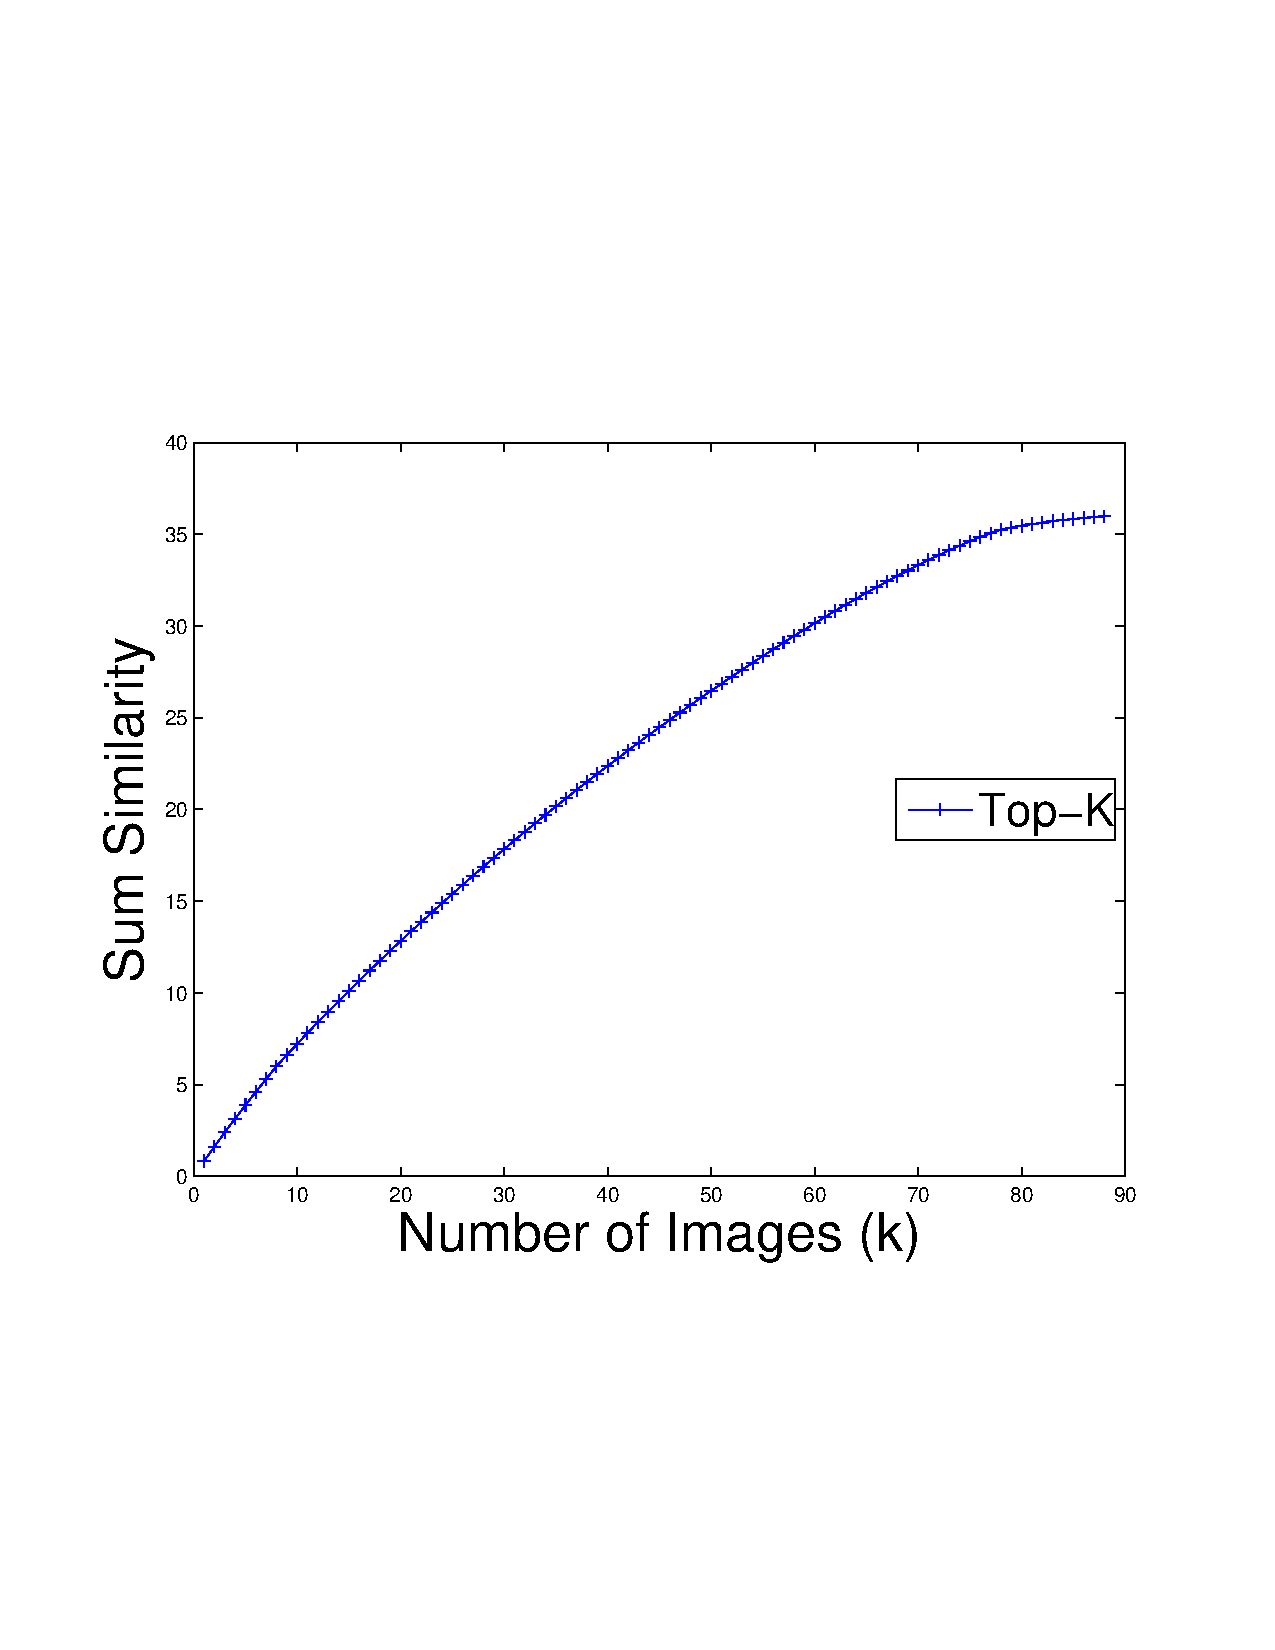
\includegraphics[clip=true, trim = 17mm 65mm 25mm 70mm, scale=0.23]{figures/topk/topk_sum_sim_color.pdf}
        \label{fig:topkSumSim}
        }
    \subfigure[Top-K: Avg. Match Target]{
        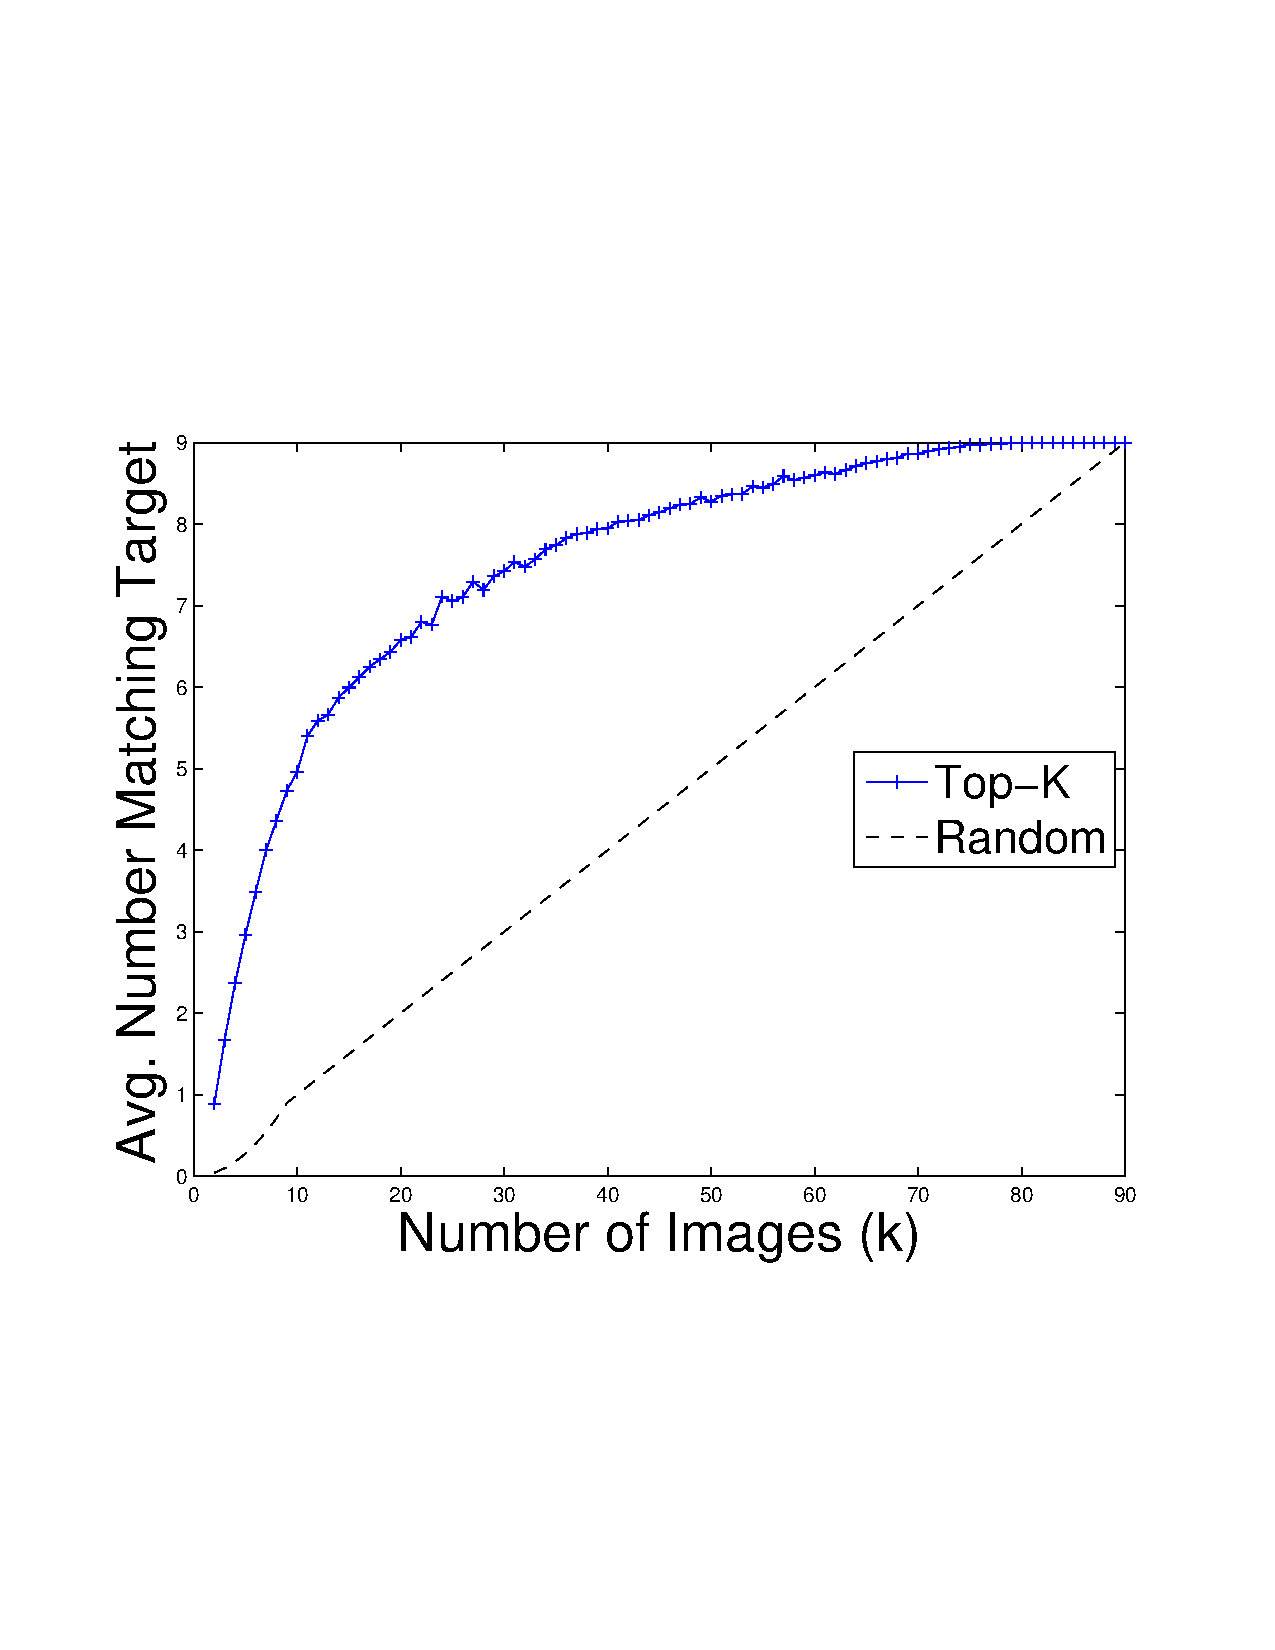
\includegraphics[clip=true, trim = 17mm 65mm 25mm 70mm, scale=0.23]{figures/topk/avg_num_matching_color.pdf}
        \label{fig:topkAvgNumSameSet}
        }
    \subfigure[Spanner: Sum Dissimilarity]{
        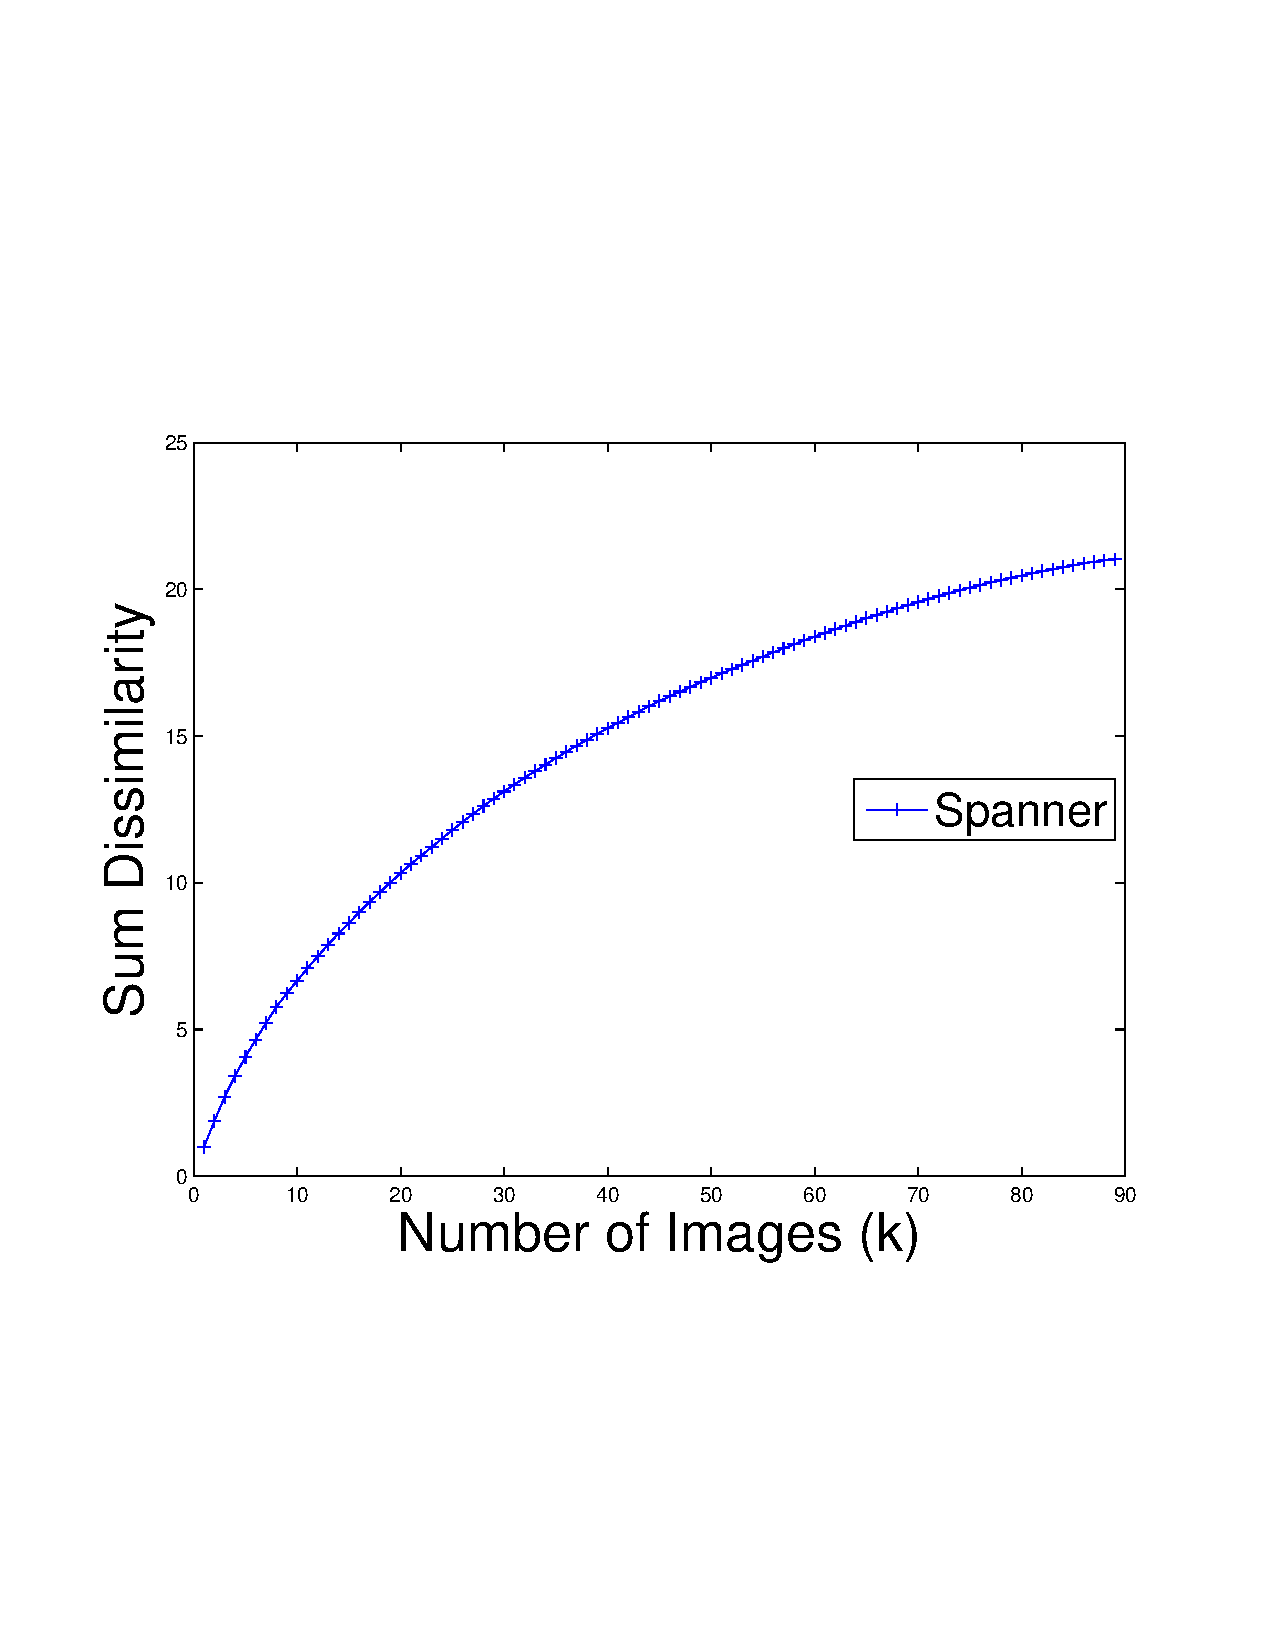
\includegraphics[clip=true, trim = 17mm 65mm 25mm 70mm, scale=0.23]{figures/spanner/spannerCumulativeDist_color.pdf}
        \label{fig:spanSumDissim}
        }
    \subfigure[Clustering: Cover All Sets]{
        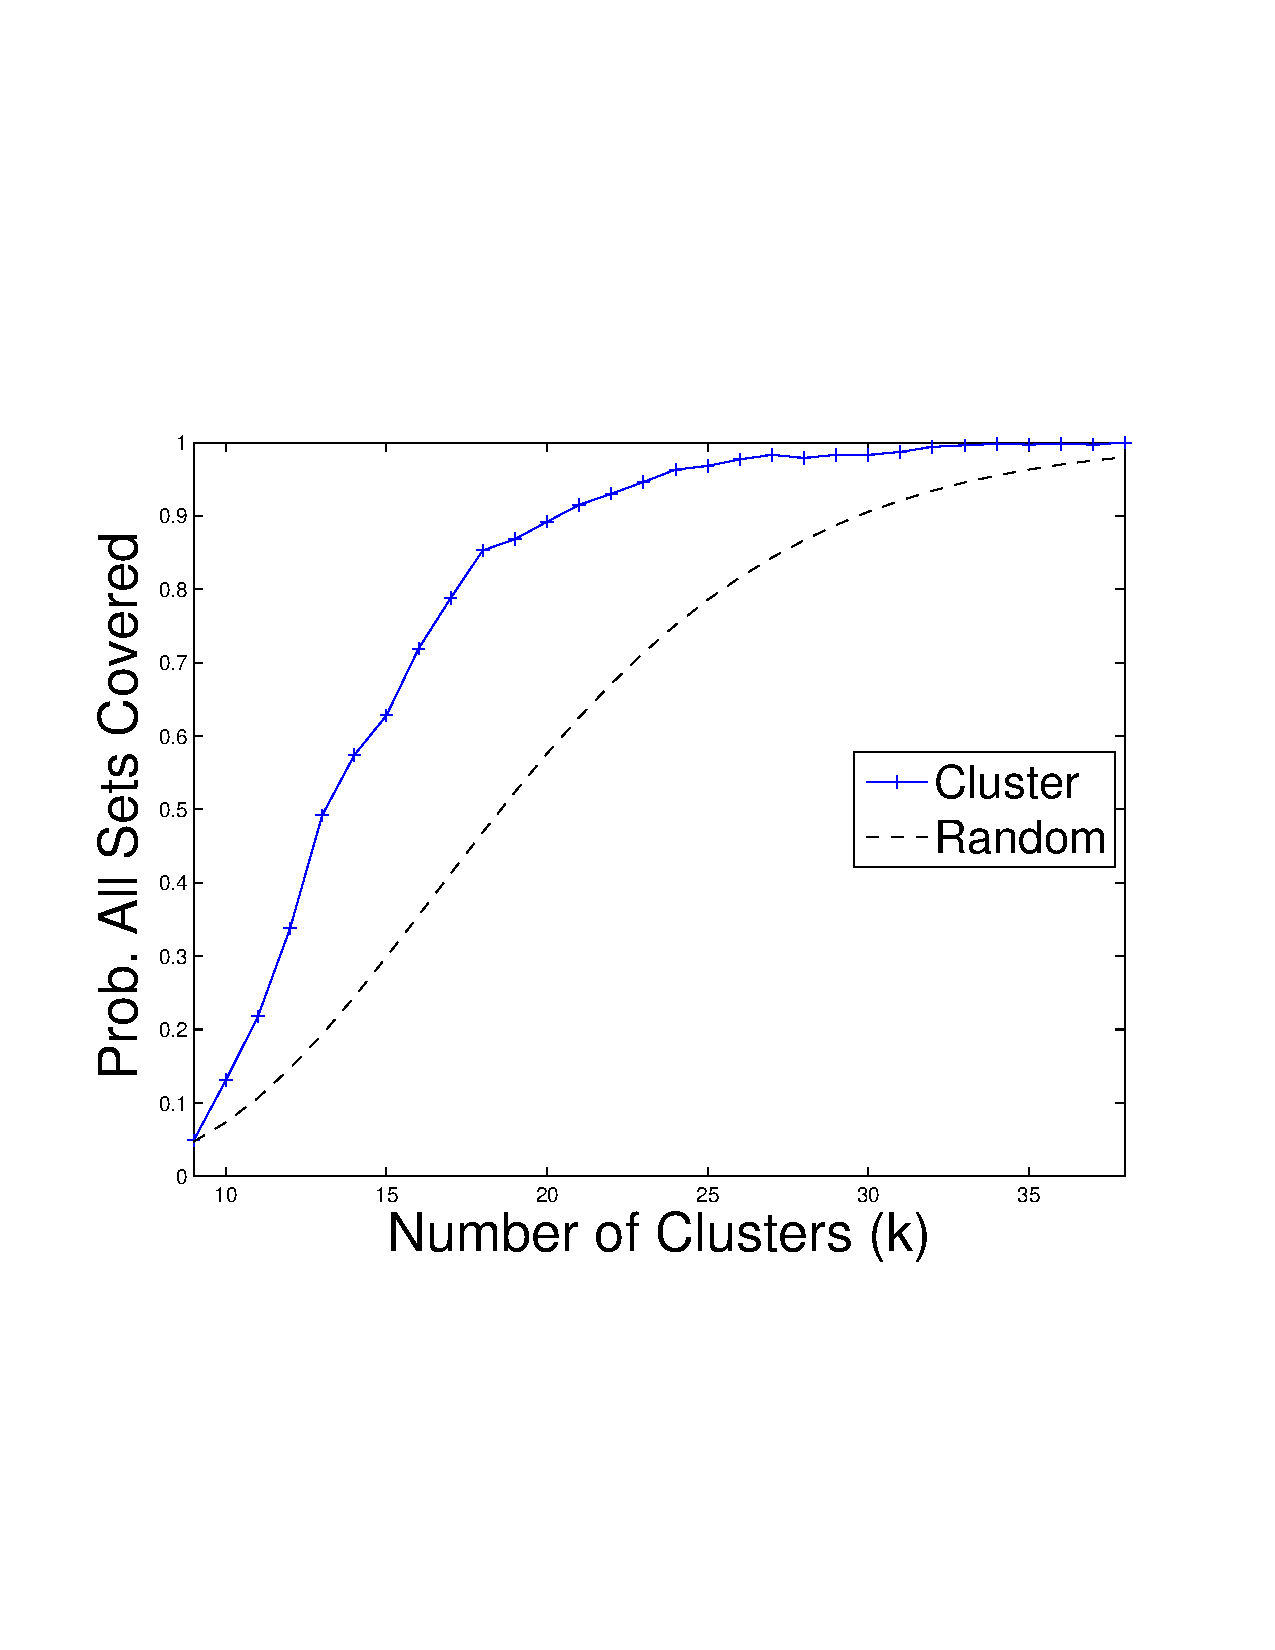
\includegraphics[clip=true, trim = 16mm 65mm 25mm 70mm, scale=0.23]{figures/cluster/perc_all_sets_covered_vary_k_color.pdf}
        \label{fig:clusterAvgNumSetsCov}
        }        
   \caption{Completeness metrics for the three image selection algorithms. Each exhibits a diminishing return as more images are added.}
   \label{fig:completeness_exp_results}
   \vspace{-4mm}
\end{figure*}

\section{QoI Model}
\label{sec:qoi_model}

%\begin{figure}
%\centering
%    \subfigure[Sum Similarity]{
%        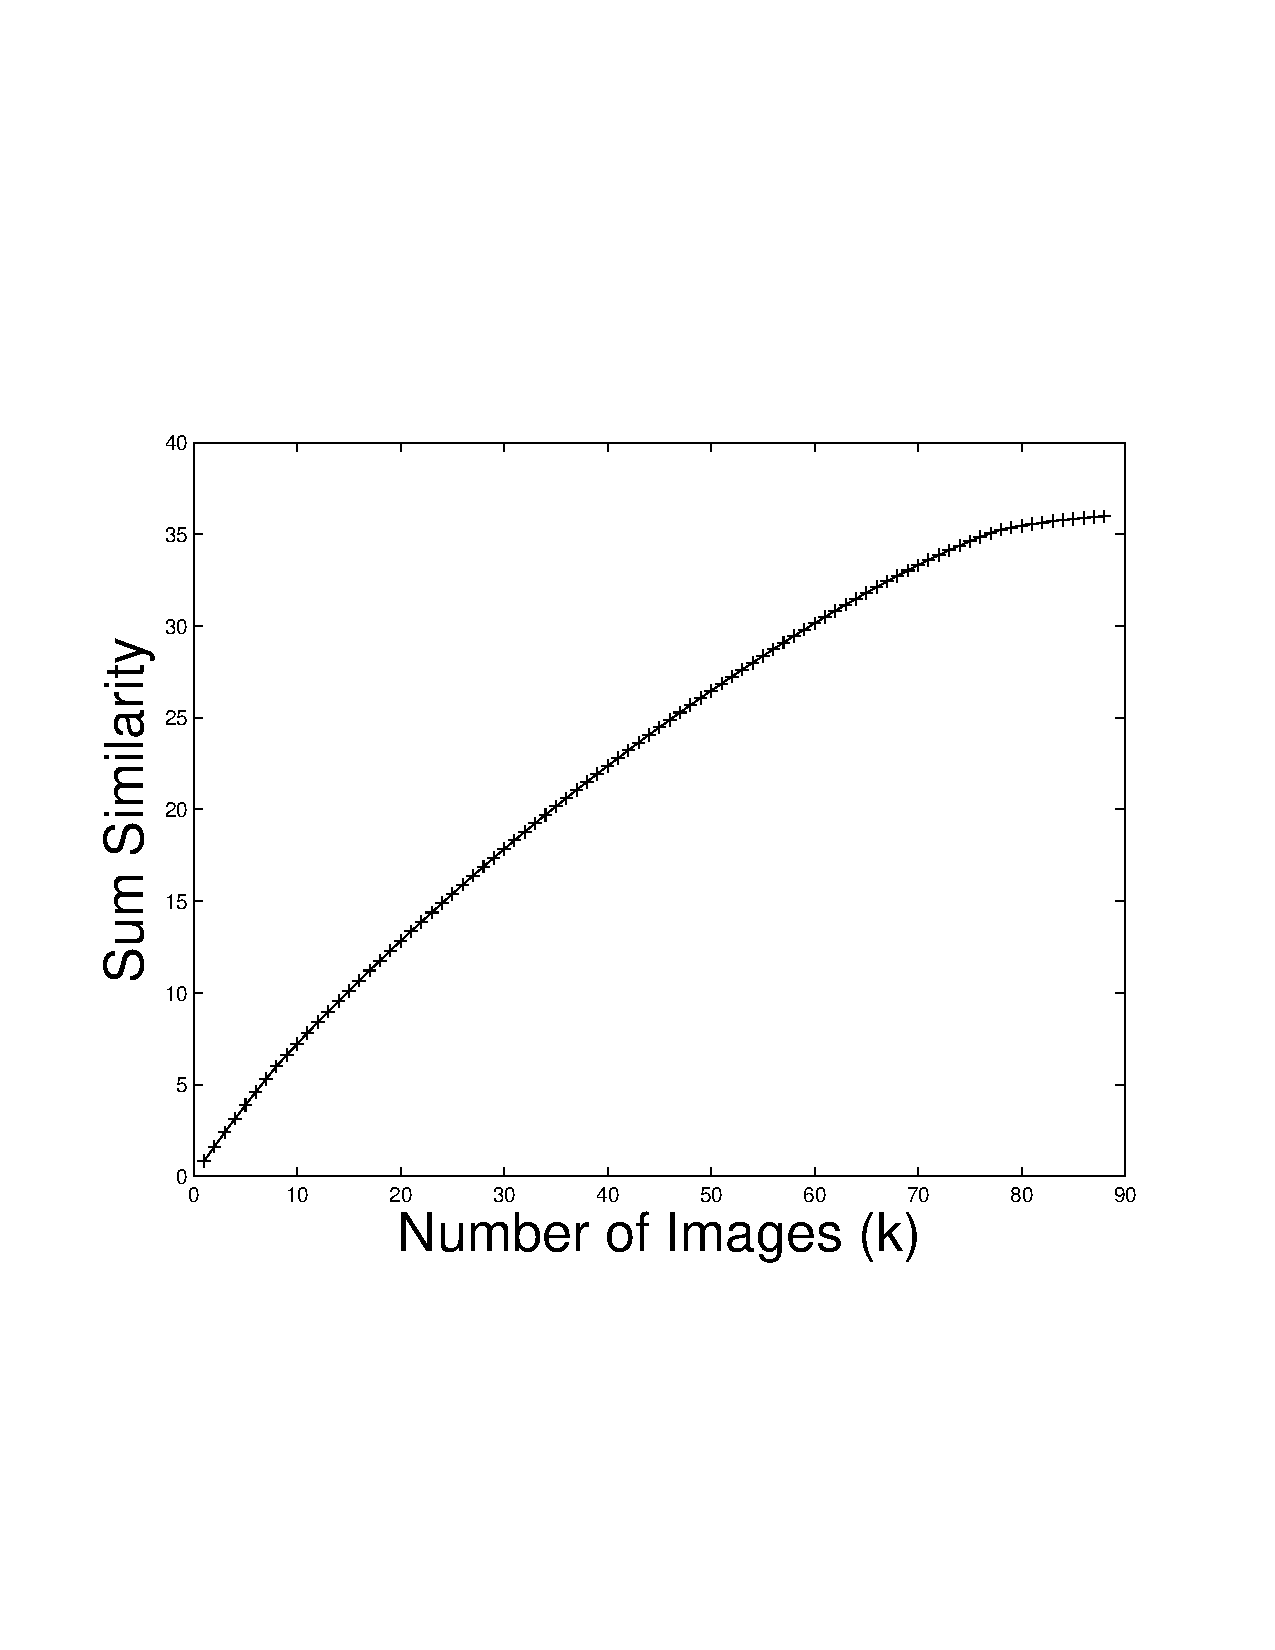
\includegraphics[clip=true, trim = 17mm 65mm 25mm 70mm, scale=0.23]{figures/topk/topk_sum_sim.pdf}
%        \label{fig:topkSumSim}
%        }
%    \subfigure[Avg. Match Target]{
%        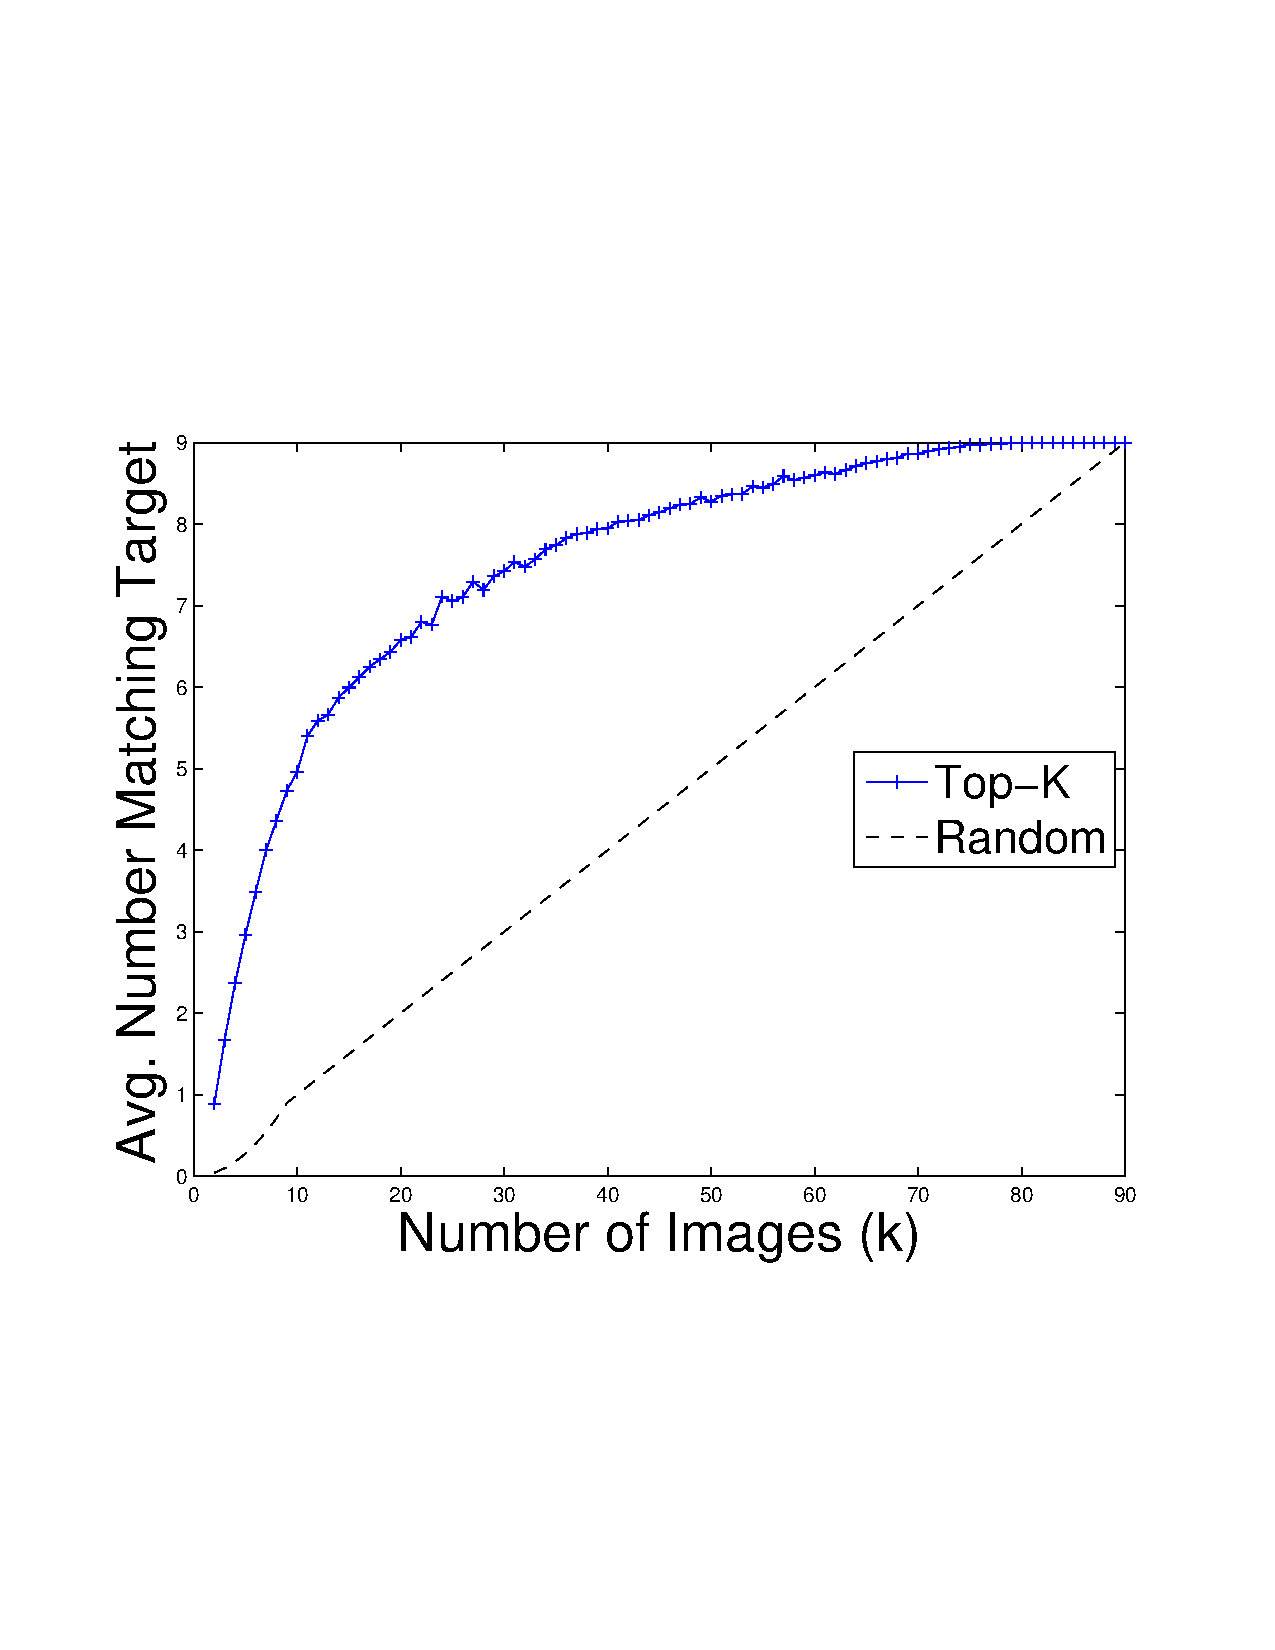
\includegraphics[clip=true, trim = 17mm 65mm 23mm 70mm, scale=0.23]{figures/topk/avg_num_matching_color.pdf}
%        \label{fig:topkAvgNumSameSet}
%        }
%   \caption{Completeness metrics for the Top-K selection algorithm. Each exhibits a diminishing return as more images are added.}
%   \label{fig:completeness_exp_results}
%\end{figure}

\begin{figure*}
\centering
    \subfigure[Top-K: Sum Similarity]{
        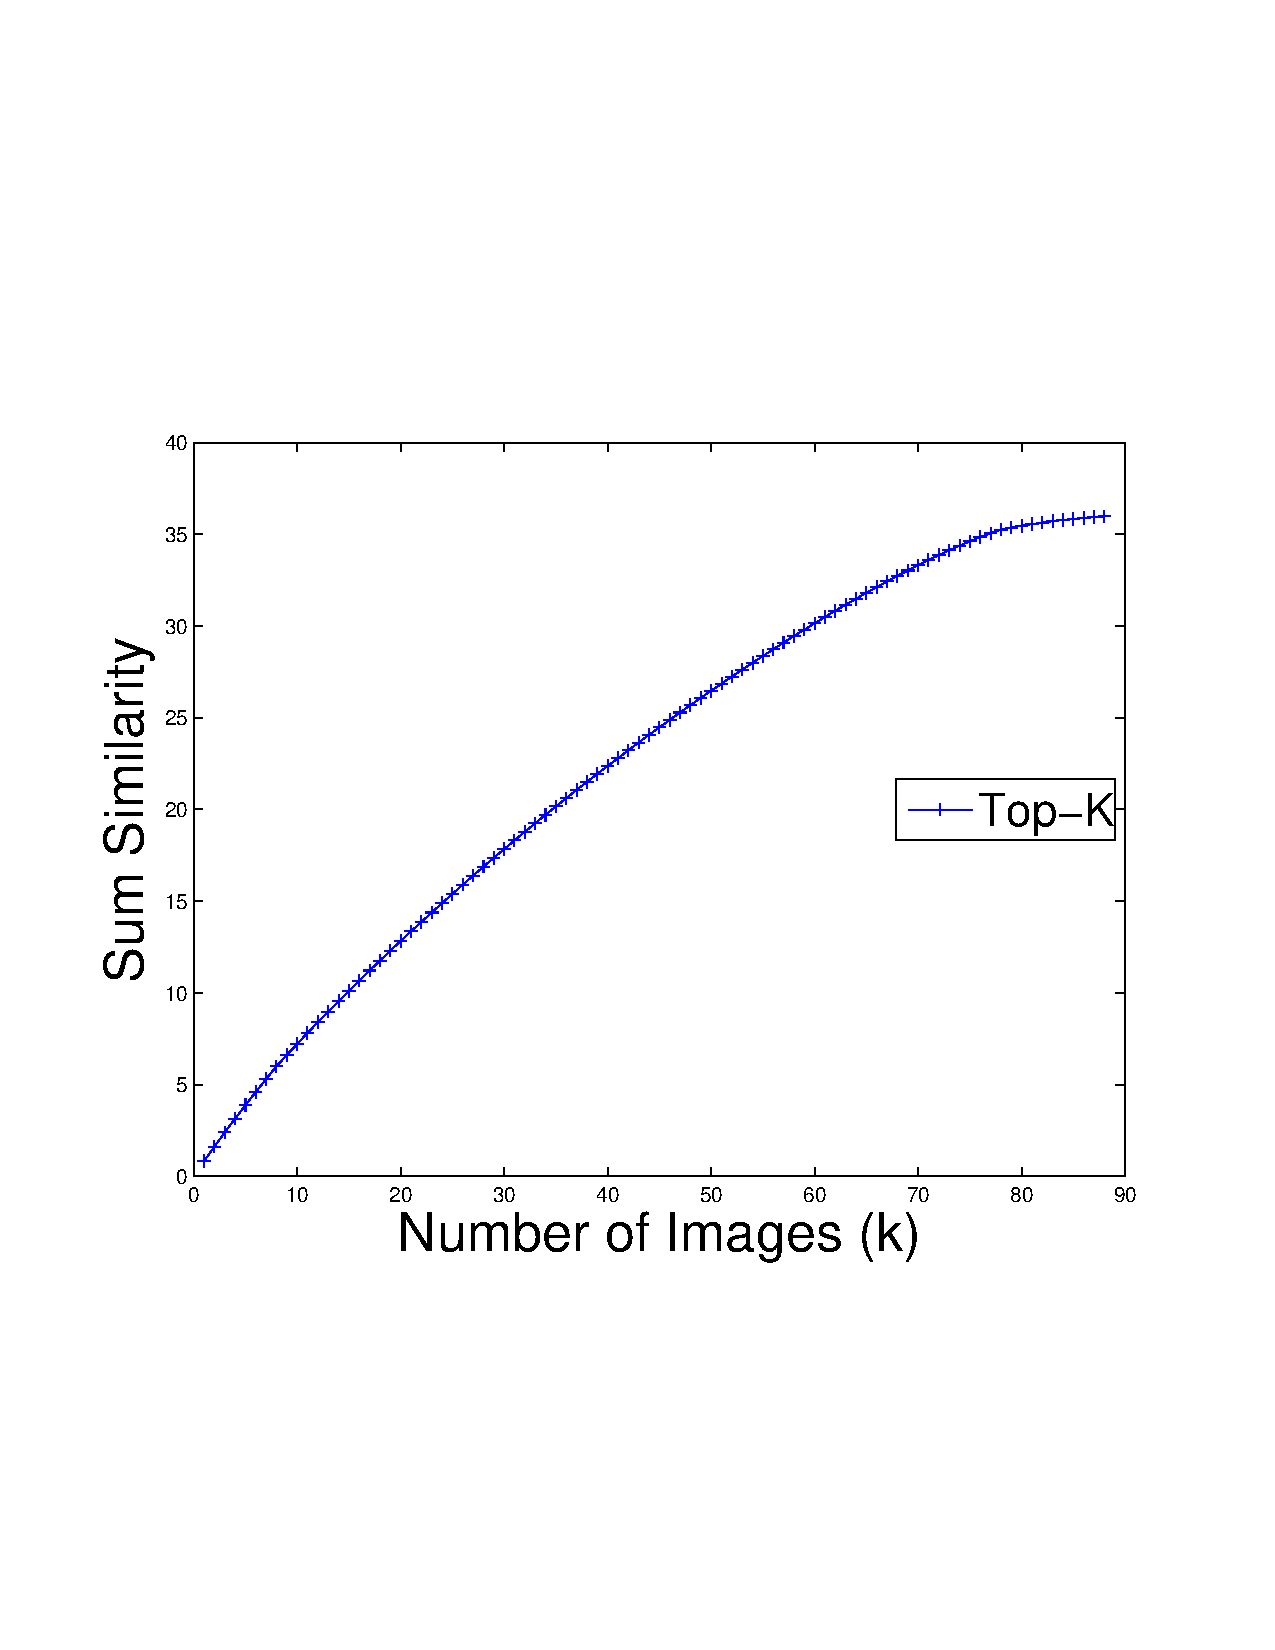
\includegraphics[clip=true, trim = 17mm 65mm 25mm 70mm, scale=0.23]{figures/topk/topk_sum_sim_color.pdf}
        \label{fig:topkSumSim}
        }
    \subfigure[Top-K: Avg. Match Target]{
        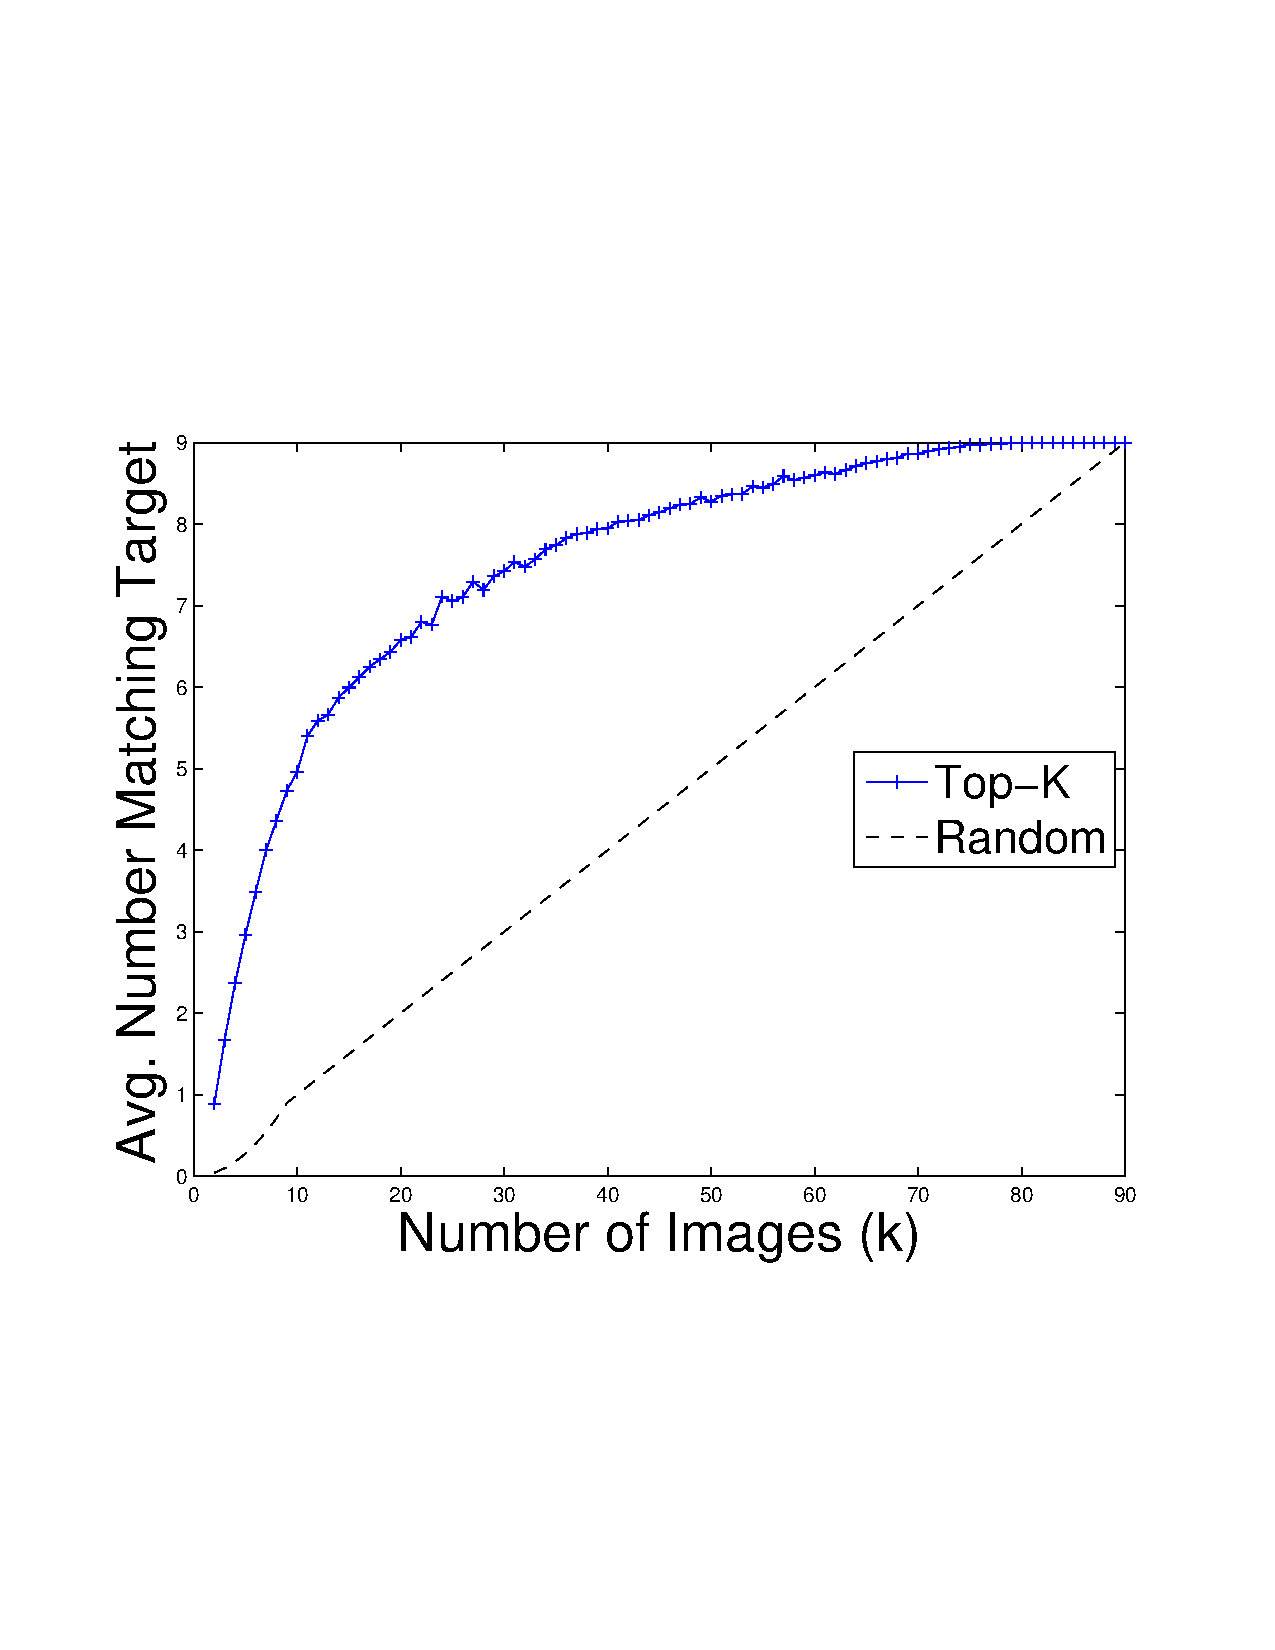
\includegraphics[clip=true, trim = 17mm 65mm 25mm 70mm, scale=0.23]{figures/topk/avg_num_matching_color.pdf}
        \label{fig:topkAvgNumSameSet}
        }
    \subfigure[Spanner: Sum Dissimilarity]{
        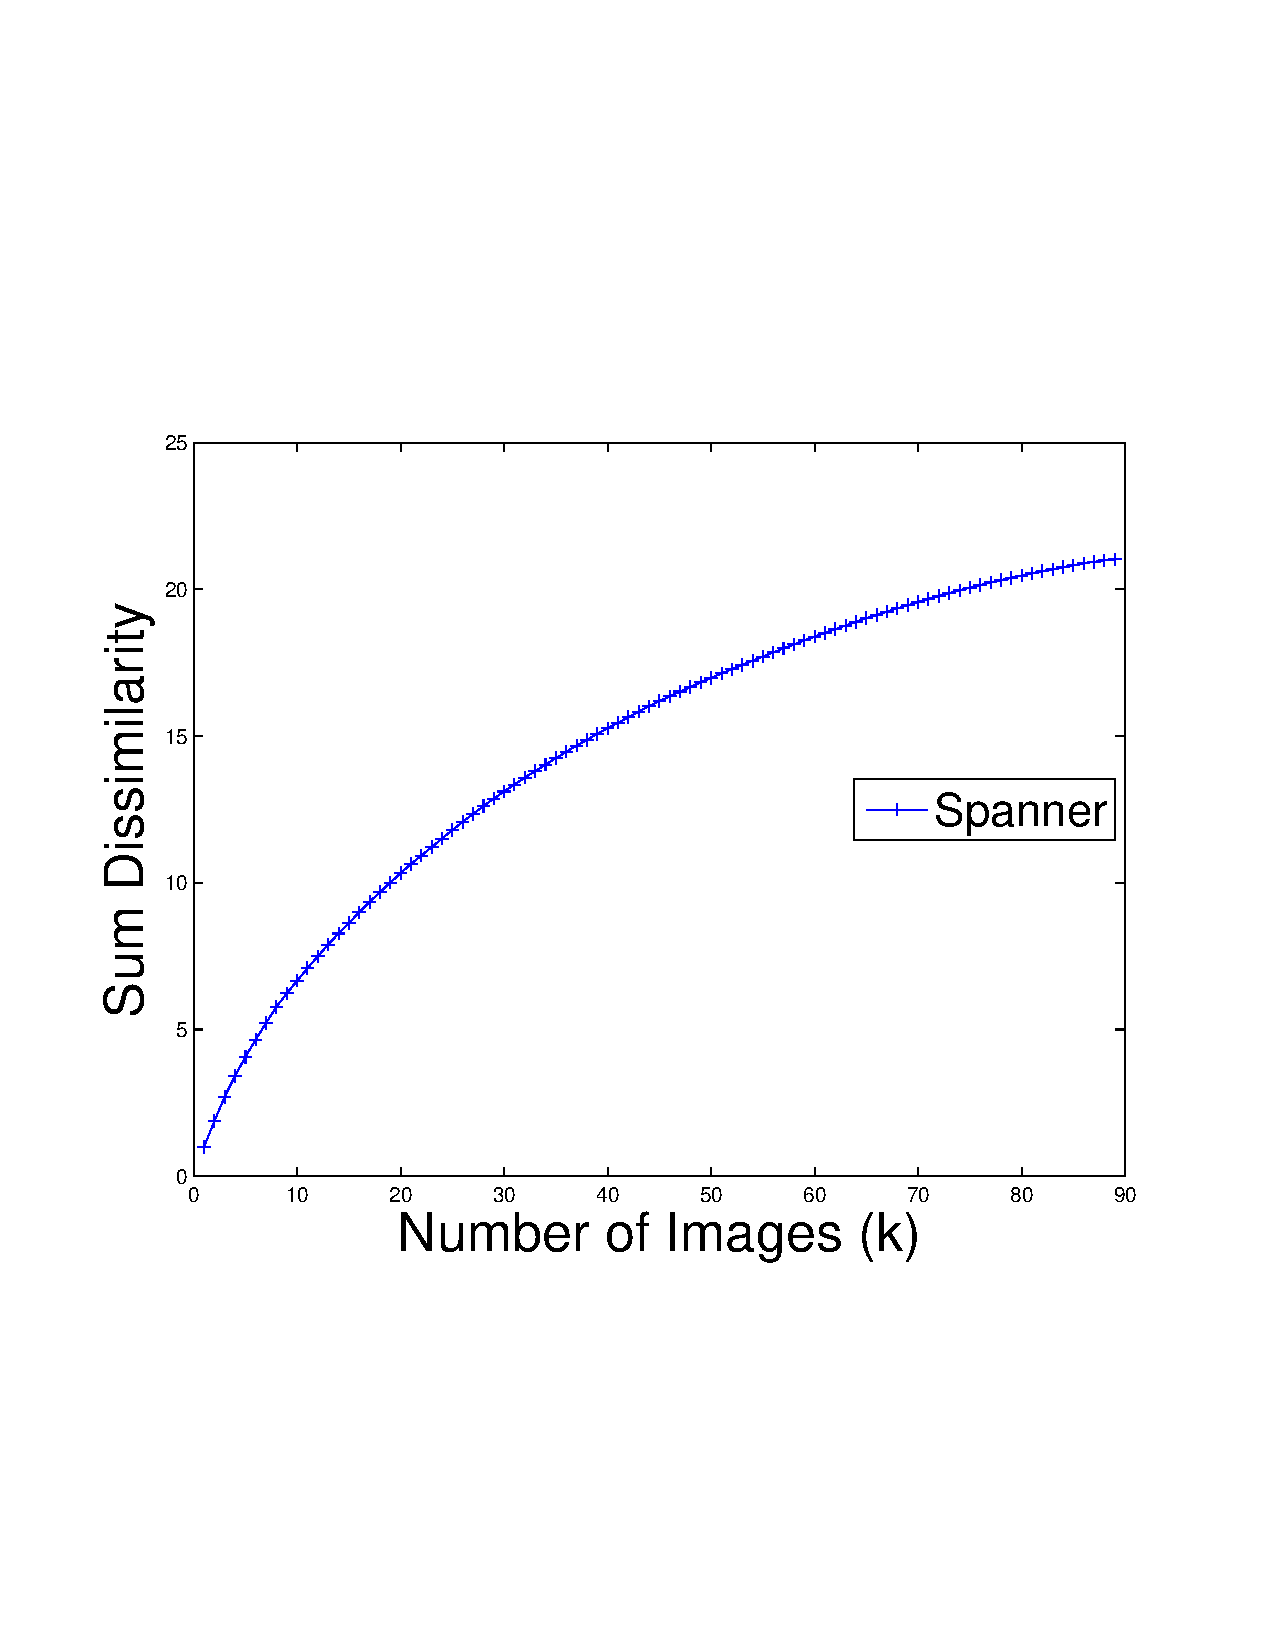
\includegraphics[clip=true, trim = 17mm 65mm 25mm 70mm, scale=0.23]{figures/spanner/spannerCumulativeDist_color.pdf}
        \label{fig:spanSumDissim}
        }
    \subfigure[Clustering: Cover All Sets]{
        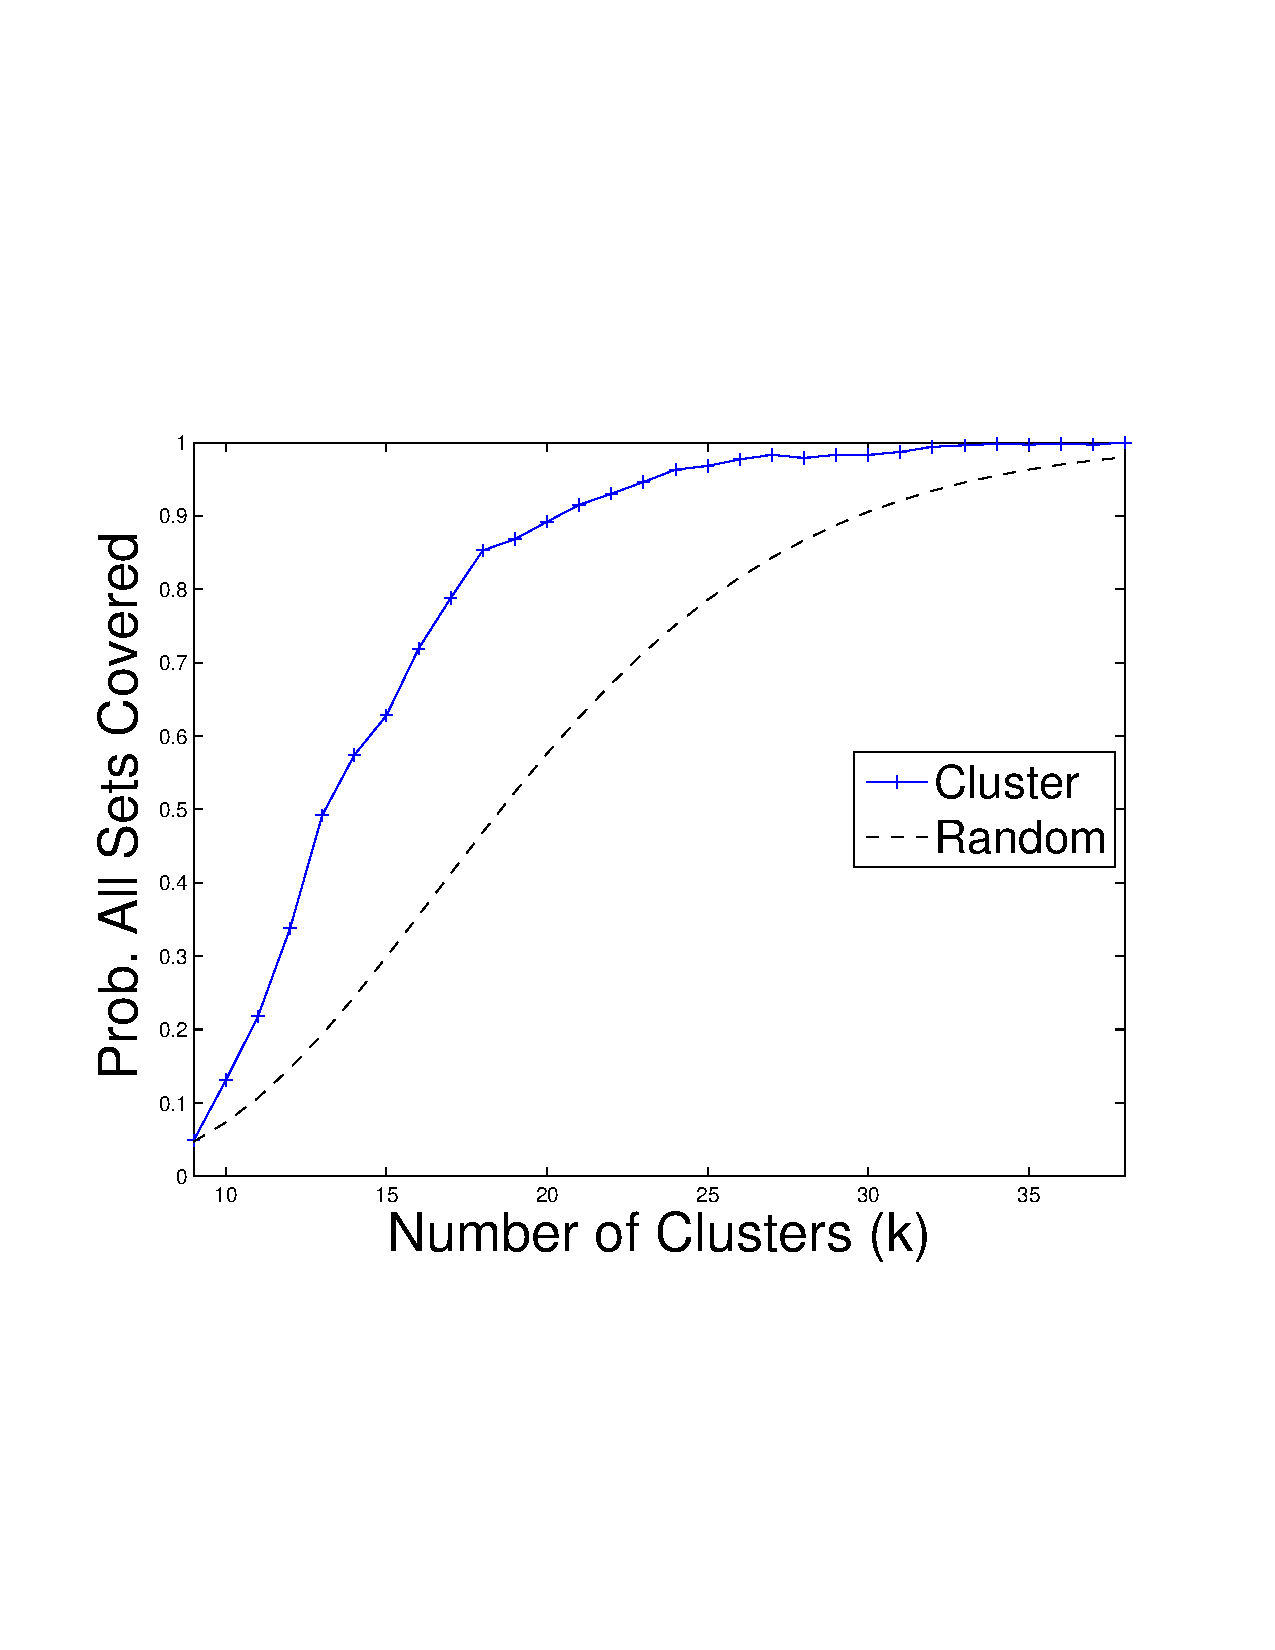
\includegraphics[clip=true, trim = 16mm 65mm 25mm 70mm, scale=0.23]{figures/cluster/perc_all_sets_covered_vary_k_color.pdf}
        \label{fig:clusterAvgNumSetsCov}
        }        
   \caption{Completeness metrics for the three image selection algorithms. Each exhibits a diminishing return as more images are added.}
   \label{fig:completeness_exp_results}
\end{figure*}

QoI is a multi-dimensional metric that can be defined for an application to give a more meaningful measure of the value of information.  It consists of attributes such as  timeliness, freshness, completeness, accuracy, precision, etc.  
For example, information that contributes to a decision-making process may only be useful if it arrives before the decision must be made, or it may have varying usefulness based on how similar or dissimilar it is to other data already collected.

The specific details of which attributes are considered and how they contribute to QoI is application-dependent.  Chosen QoI metrics are stored as a vector associated with a data item.  
Here, as in \cite{qoi_aware_tactical_mil_nets}, we specify a vector of minimum values for each QoI metric, and 
information is evaluated based on whether it satisfies all of the QoI requirements or not.  We use this approach to establish the edges of QoI satisfiability for the vector of metrics, which defines the boundaries of maximum achievable QoI regions in the metric space.

We choose to use two QoI attributes, one that is time-based and one that is information-content-based.  The first attribute is timeliness, $T$, of data.  For the second attribute, we present a notion of \emph{completeness}, $C$, which we show can be defined multiple ways, depending on the application and context.  Together, a QoI requirement of $\mathbf{q} = \{C,T\}$ specifies a quantity of data that must be delivered as well as a deadline by which it must arrive to be useful.  Since completeness is a rather new concept, we explain an example image selection algorithm and show how it can be evaluated with completeness.
%REFERENCES THAT USE COMPLETENESS: 1) mentions completeness of information in context of mobile sensor networks; argues that mobility can increase coverage/completeness \cite{qoi_data_collection_mobile_sens_nets};  

\subsection{Example Application: Similarity-based Image Retrieval}

As a motivating example, we choose a network in which nodes store photographs that are to be exchanged or collected at one or more data sinks.  This example covers surveillance missions of military tactical networks or camera sensor networks.  In this model, nodes can act as both clients and servers, issuing queries and serving images in response.  Therefore, as the network size increases, the amount of traffic is also likely to increase, but possibly disproportionately.  This fact exemplifies why the problem of characterizing the scalability limits for an instance is not straightforward.

To satisfy completeness of a query, we utilize measurements of the similarity or dissimilarity between pairs of images as explained in the rest of this section.  To get a similarity measurement, we use the same choice as was shown to be effective in \cite{mediascope}.  A technique called Color and Edge Directivity Descriptor (CEDD) \cite{2008cedd} provides a $54$-byte vector of qualities inherent to a photograph like lightness, contrast, and color.  The similarity between two images can then be given as a scalar by calculating the \emph{Tanimoto Similarity} \cite{tanimoto} between their CEDD vectors.  Dissimilarity is simply defined as $1$ minus the similarity.

\subsubsection{Selecting Similar Images}
One possible query for data is to retrieve images from the network that are similar to an identified target image.
The first type of query we introduce occurs when a user already has one image of a particular area or object of interest and would like to obtain similar images to get a more complete view of that specific scene or object.  
For example, if a user has a picture of an unknown suspicious person entering a building, but the person is not identifiable from that image, it would be useful to collect more images that are similar to that one with the possibility that another picture may have a better view of the person in question that can be used for identification or more context.  Called {\bf Top-K}, the query algorithm used for this application will choose the $k$ images with the most similarity with respect to the target image.  

We can evaluate the completeness of the result in one of two ways.  First, we can use the similarity of the images as a value representing each image's effectiveness in providing a more complete view of the target scene.  If we sum the similarity of all $k$ images returned by the algorithm, we get a representation of completeness, which we naturally call \emph{Sum Similarity}.  While this measure of completeness is abstract, it can be refined in an actual implementation through testing and evaluating.  This definition of completeness is useful, though, because it can be applied without any predetermined knowledge of the environment or pool of images.  

Often, though, we can partition the environment in which the network operates into a number, $n$, of distinct settings or areas.  In those cases, we can utilize a second method of quantifying completeness.  Assume that each image belongs to one of these $n$ sets, %$Q_i$, 
related to the setting it depicts.  Naturally, then, when executing a Top-K query, the goal is for the algorithm to return images from the same set as the target image.  Completeness can then be given by the fraction of images returned that are in the same set as the target image.

\subsubsection{Selecting Diverse Images}

In contrast, given the set of all photographs available in the network, we might want to return the set of $k$ images that exhibits the most diversity, ideally providing a user with a good sampling, or \emph{complete view}, of available images.  For instance, such a result would be quite useful in a surveillance mission.  We present two query algorithms that can be used to achieve this goal.

One query that provides diverse images is known as the {\bf Spanner} of the set of known photographs.  For the Spanner algorithm, we employ a greedy algorithm similar to that in \cite{mediascope}.  Here, the algorithm simply chooses images that provide the greatest minimum distance from all images already chosen.  This minimum distance can be added to a running sum to provide a completeness metric of \emph{Sum Dissimilarity}.  This value represents a measure of completeness because a higher level of dissimilarity provides a more complete view of the feature space.

%Here, the algorithm first chooses the two images with the greatest dissimilarity between them from all available images.  Then, each successive image is chosen to be the one with the greatest minimum distance between it and all images already chosen, until $k$ images are selected.  This minimum distance between the image being selected and the images in the collected set is the value added to the running cumulative completeness metric of \emph{Sum Dissimilarity}.  Since the Spanner algorithm's goal is to provide images at the edges of the available feature space, the Sum Dissimilarity represents a measure of its completeness because a higher level of dissimilarity is providing a more complete view of the feature space.

The other query that can achieve a complete view over all images is {\bf Clustering}.  In the Clustering algorithm, all images are separated into $k$ clusters based on their pairwise distances using any version of a k-means clustering algorithm, where $k$ is given by the user.  Then, the most central image from each cluster is returned.  
Here, assuming that the photographs of the same settings or objects of interest exhibit similar characteristics, 
Clustering also provides a complete view of the network's environment.

Both Spanner and Clustering algorithms can also be evaluated using a model assuming the environment is split into $n$ sets.  With this model, we can define completeness as either the number of sets represented by at least one of the $k$ images returned or the probability of all $n$ sets being represented by at least one image when $k$ are returned.  Here, though, we only show results for the second definition.

\subsection{Experimental Results}

To provide example values of these completeness metric definitions, experiments applying each query algorithm were run on a set of pictures taken at $n = 9$ different settings around the Penn State campus.  Each of these $9$ settings is of a pictorially different area, e.g. a particular building, a downtown street, or a lawn setting, and over $20$ images of each was taken.  Then, for individual trials, $10$ images from each set were randomly selected to create an image pool of $90$ pictures.  The three algorithms were run over these $90$ images, with the target image being randomly selected in the case of Top-K.  Results for each of the different completeness metrics were averaged over $1,000$ trials are shown in Figure \ref{fig:completeness_exp_results}. % Figures \ref{fig:topkSumSim} to \ref{fig:clusterAvgNumSetsCov}.

Figure \ref{fig:topkSumSim} shows the average sum similarity of images returned by the Top-K algorithm.  Figure \ref{fig:topkAvgNumSameSet} provides the second definition of completeness for the Top-K algorithm, the number of images matching the set that the target image was randomly chosen from.  Completeness results when dissimilarity is the objective are shown in Figures \ref{fig:spanSumDissim} and \ref{fig:clusterAvgNumSetsCov}.  Specifically, Figure \ref{fig:spanSumDissim} depicts the average Sum Dissimilarity returned by the Spanner algorithm, and Figure \ref{fig:clusterAvgNumSetsCov} represents the empirical probability of all $9$ sets being represented in the $k$ returned images.   For reference, we also include expected values for the metrics in Figures \ref{fig:topkAvgNumSameSet} and \ref{fig:clusterAvgNumSetsCov} if the images were selected from the entire image pool at random, i.e., without regard for image similarity or dissimilarity.  Details on these expected values given random selection are in Appendix \ref{sec:expl_exp_qoi}.

These figures exhibit the diminishing returns of completeness as more images are collected.  This effect visually shows how QoI differs from throughput.  As seen in these graphs, transmission of successive images does not result in a linear gain in completeness.  For example, in Figure \ref{fig:topkAvgNumSameSet}, it is evident that a value of only $k \approx 10$ is needed to collect $5$ images matching the target content, while collecting an additional $2$ from the same set usually requires collecting over twice that number of pictures.  
%For comparison, Figure \ref{fig:topkAvgNumSameSet} also shows the completeness achieved by random selection.
Similarly, Figure \ref{fig:clusterAvgNumSetsCov} shows that jumping from $k=10$ to $k=20$, the likelihood of capturing at least one image of every setting grows substantially from just over $10\%$ to approximately $90\%$.  To approach probabilities close to gaining that final $10\%$, however, requires a jump to $k\approx30$.  

The relationship between the number of images and completeness in each of these graphs also shows that obtaining a certain value of QoI or completeness requires a different number of images depending on the set available and their similarities.  We can denote the number of images required to achieve a level of completeness, $C$, as $k_{req} = Q(C)$.  This relationship will be useful later in determining capacity and scalability limits.

%\subsection{Other Applications}
%In our work, we also studied and experimented with two other algorithms in \cite{mediascope} that provide completeness by returning images that are dissimilar from each, providing a representative view of available data.  These completeness definitions resulted in very similar relationships as seen in Figure \ref{fig:completeness_exp_results} and are omitted for space.  We also note that the formulation in Section \ref{sec:qoi_scalability} is not restricted to just completeness, but can be used with any QoI metric that can be translated into a data requirement.
\subsection{Further Discussion of QoI}
We have defined and provided examples for a number of ways that completeness can be defined and used to obtain a concrete data requirement from a contextual QoI requirement.  Throughout the rest of the paper, we use sum similarity and the probability of covering all sets using clustering as completeness metrics, but we note that any of the definitions of completeness used here, or any other QoI requirement that can be translated into a data requirement, for that matter, can be used. % in the formulation in Section \ref{sec:qoi_scalability}.

%Also, note that QoI and its usage in understanding networks is not exclusive to these metrics and applications.  On the contrary, the model used in the capacity and scalability analysis of Section \ref{sec:qoi_scalability} is meant to be an in-depth example of this concept.  Modifications to account for different data size requirements should be quite straightforward, and extensions to other time-based metrics should be possible with careful extensions to the framework.

Also, while metadata associated with photographs may be useful in obtaining similar goals to those given in this section, relying on such information is problematic because metadata is not guaranteed to be available, and it is not as universally applicable as content-based retrieval.  For example, tags describing the image contents would require users to participate by entering this information, which is time-consuming and unreliable.  Location and time stamps may be automatically applied by the device allowing an application to filter images accordingly, but these tags often do not account for factors such as the direction of the camera or obstructed views.  Content-based processing, though, can be applied to any set of images.





\section{Finding Bottleneck Flow}
\label{sec:bottleneck}

Again, we turn to the satisfiability equation, but use random variables for the Traffic Factor and Path Length, $TF_i$ and $PL_i$, respectively:
\begin{equation}
	T \geq \frac{ k_{req} \cdot I_S \cdot CF \cdot TF_i}{W} + \frac{P_S \cdot DF \cdot (PL_i-1)}{W}
\end{equation}
where we will call the total delay
\begin{equation}
	D_i = \frac{ k_{req} \cdot I_S \cdot CF \cdot TF_i}{W} + \frac{P_S \cdot DF \cdot (PL_i-1)}{W}
\end{equation}

Now, we want to identify which flow $i$, identified by its origin node, is most likely to be the flow that cannot be satisfied in the allotted timeliness.  To do so, we can simply find the value of $i$ that results in the largest $D_i$.

\begin{figure}
\begin{centering}
    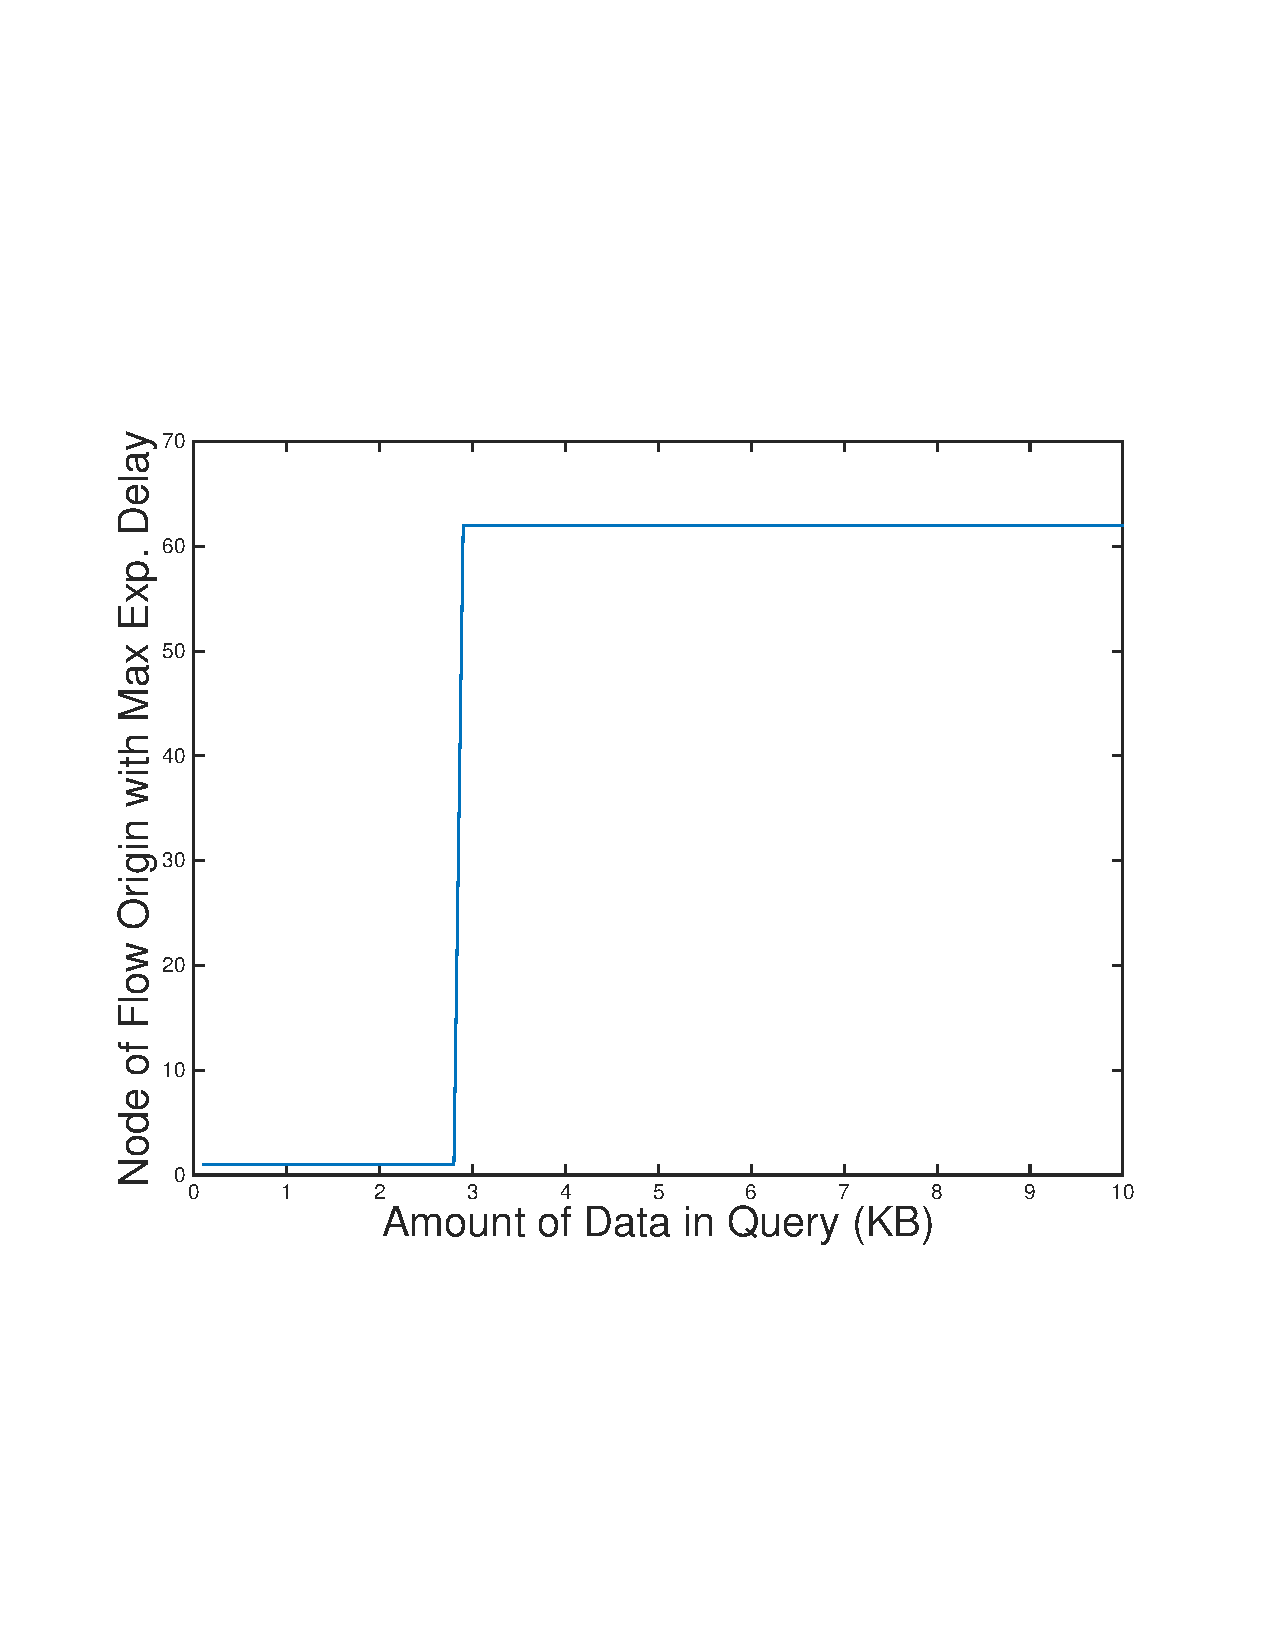
\includegraphics[scale=0.4, clip=true, trim=15mm 65mm 20mm 65mm]{figures/max_i_line_net_125.pdf}
    \caption{The value of $i$ (origin of a flow) that causes the maximum expected delay.}
    \label{fig:max_i_line_net}
\end{centering}
\end{figure}

Using the expected values for $TF_i$ and $PL_i$ from Figures \ref{fig:EV_TF_line_net} and \ref{fig:mean_PL_each_node_line_net}, we find the value of $i$ that maximizes $D_i$ for different data requirements, $B = k_{req}*I_S$.  Figure \ref{fig:max_i_line_net} shows that for low data requirements, the delay of multi-hop paths dominates, causing the ``Bottleneck" flow to be those that originate in node $1$ and have a larger expected path length.  At a point, though, as the amount of data required in the query grows, congestion will be the limiting factor in the network, making the Traffic Factor more important.  Thus, the node near the center of the network which will be likely to experience the highest amount of congestion become the source of flows with the highest delay.  In this case, we have $i = 62$, since the network has $125$ nodes (NOTE: It should probably be 63, but there is an ``off-by-one" error here because the definitions/formulations are not carefully derived to be correct on the boundaries).



%\section{Probability of Satisfying Query}
\label{sec:prob_sat}

Now, we have an expression for delay that is built up using random variables for the values of $TF$ and $PL$.  The next useful formulation is providing an expression that describes the probability of a bottleneck flow satisfying its timeliness requirement considering the underlying distributions.  With this formulation, we can define scalability as a network in which the flow's probability of satisfiability exceeds some threshold $P_{thresh}$:
\begin{equation}
	P(D_i < T) \geq P_{thresh}
\end{equation}

Once again, we have our total delay equation of a flow originating in node $i$:
\begin{equation}
	D_i = \frac{ k_{req} \cdot I_S \cdot CF \cdot TF_i}{W} + \frac{P_S \cdot DF \cdot (PL_i-1)}{W}
\end{equation}
Let us define two constants to simplify the expression:
\begin{eqnarray*}
	C_1 = \frac{k_{req} \cdot I_S \cdot CF}{W} \\
	C_2 = \frac{P_S \cdot DF}{W}
\end{eqnarray*}
Then, we can express the delay as
\begin{equation}
	D_i = C_1 \cdot TF_i + C_2 \cdot PL_i
\end{equation}
As we showed in the last section, we can determine $i$ using the expected values for $TF_i$ and $PL_i$, so assuming that we adopt this value of $i$, we can drop the notation:
\begin{equation}
	D = C_1 \cdot TF + C_2 \cdot PL
\end{equation}

\begin{eqnarray}
\nonumber
	f_{TF}^i (tf) = &&\frac{i}{N} \cdot \mathcal{N}(\mu(i),\sigma(i))  \\ \nonumber
			   &+& \sum\limits_{k=i}^{\frac{N}{2}-1} \cdot \frac{\frac{1}{2}-\frac{i}{N}}{\frac{N}{2} - i}\mathcal{N}(\mu(k),\sigma(k))  \\
			   &+& \frac{1}{2} \cdot \mathcal{N} (\mu(\frac{N}{2}),\sigma(\frac{N}{2}))
\label{eq:full_PDF_TF}
\end{eqnarray}











%\begin{figure}
%\begin{centering}
%    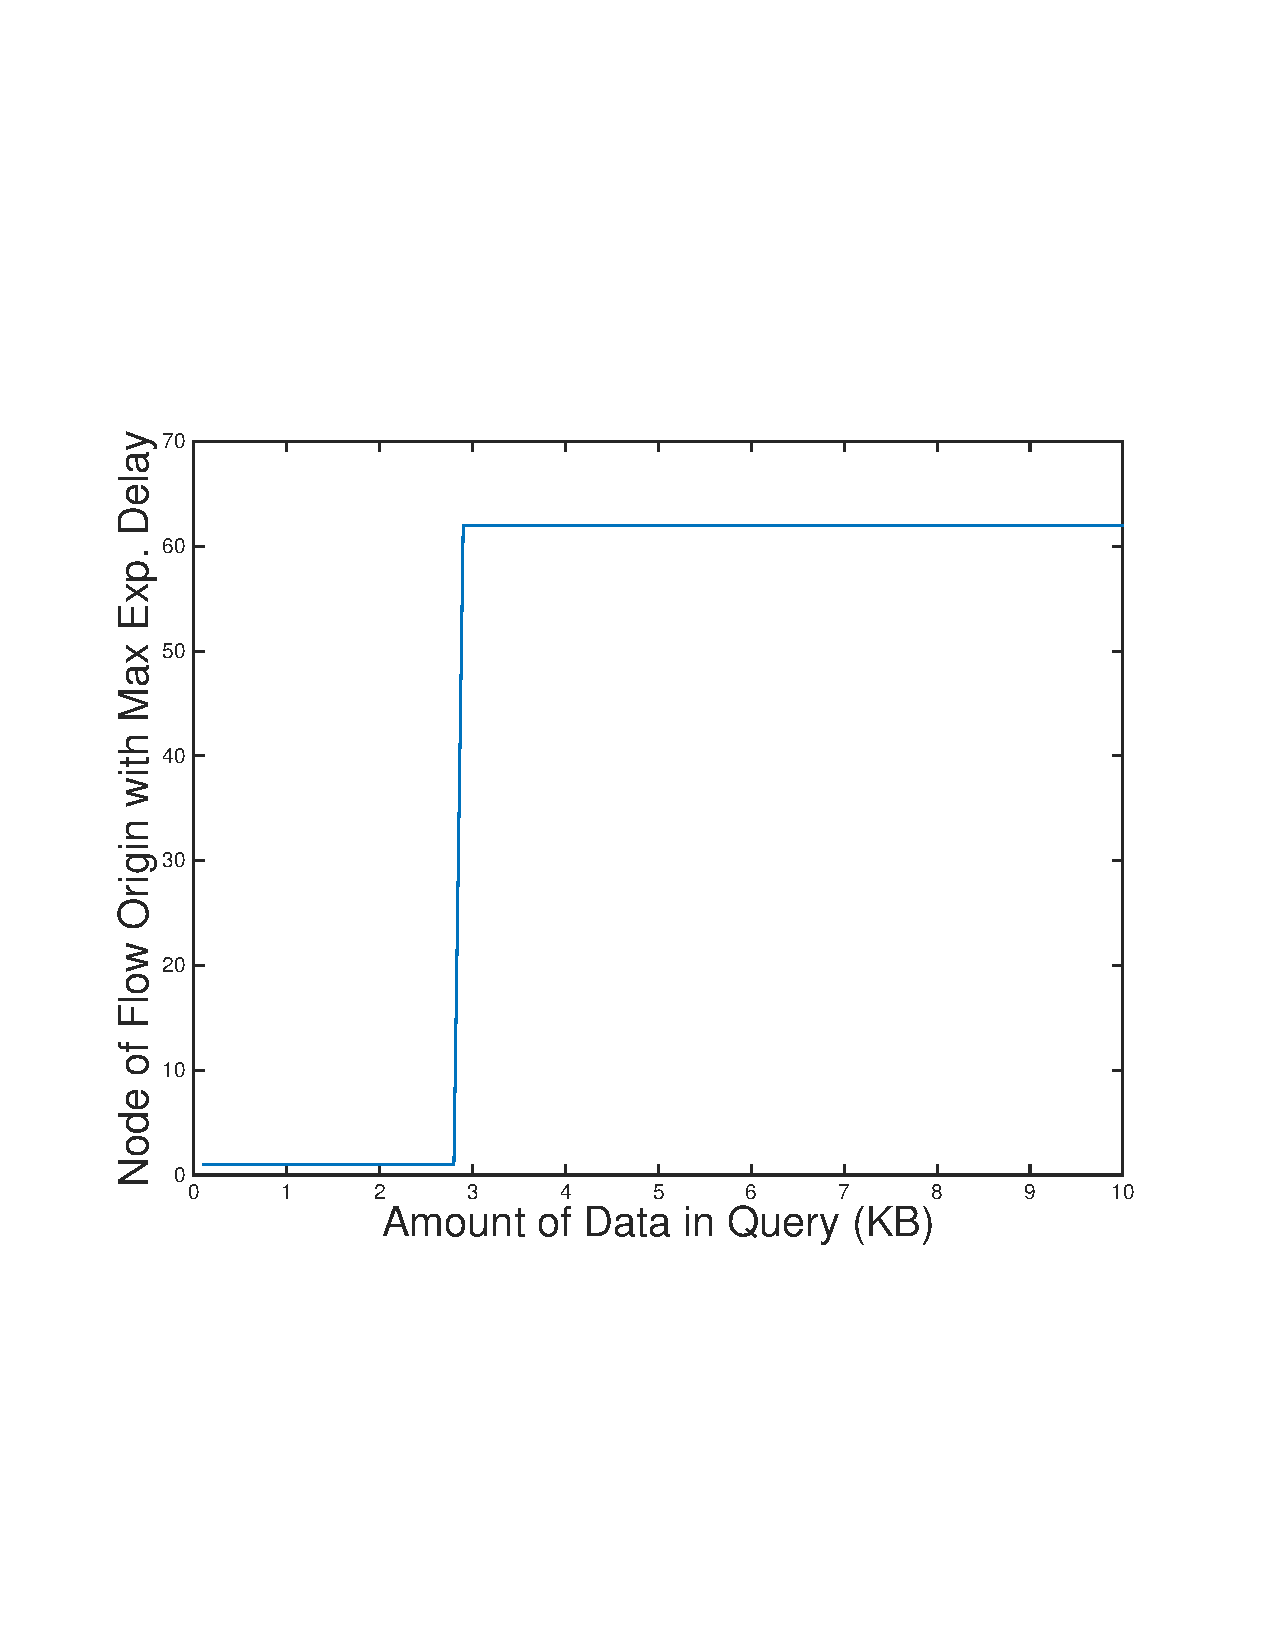
\includegraphics[scale=0.4, clip=true, trim=15mm 65mm 20mm 65mm]{figures/max_i_line_net_125.pdf}
%    \caption{The value of $i$ (origin of a flow) that causes the maximum expected delay.}
%    \label{fig:max_i_line_net}
%\end{centering}
%\end{figure}




%\section{Conclusion}
\label{sec:conclusion}

% Problem
This work provides several contributions to the field of QoI-aware wireless networks.  
%In this work, we examined network capacity and design with explicit Quality of Information consideration from a practical standpoint.
% Solution
% method and results
First, we motivated the use of completeness and timeliness as QoI attributes, providing an example application and several different ways to measure completeness.  
%We support this motivation with results from running these image selection algorithms on a real data set.
Next, we developed a framework that can be used to predict QoI and network size limits for a specific network as well as predict expected probabilities of satisfying timeliness constraints beyond the point in which all queries are satisfied.  We validated these models' accuracy by comparing analytical results with simulations performed in the ns3 network simulator in both cases.
% Take away : Lesson
Examples of the impact of different network parameters were shown, providing concrete examples of the framework's usefulness in real-world applications.  In addition, the concept of scalably feasible QoI regions was introduced.
% Future work
For future work, we plan to make generalizations of factors that will allow for easy application of this framework to any non-regular network topology and expand this framework to include consideration of more complex network control actions, such as caching and/or data compression or fusion, which are all of interest in QoI-aware networking.




%\appendix
%\input{sections/random_explanation}
% conference papers do not normally have an appendix


% use section* for acknowledgement
%\section*{Acknowledgment}


%The authors would like to thank...


% trigger a \newpage just before the given reference
% number - used to balance the columns on the last page
% adjust value as needed - may need to be readjusted if
% the document is modified later
%\IEEEtriggeratref{8}
% The "triggered" command can be changed if desired:
%\IEEEtriggercmd{\enlargethispage{-5in}}

% references section

% can use a bibliography generated by BibTeX as a .bbl file
% BibTeX documentation can be easily obtained at:
% http://www.ctan.org/tex-archive/biblio/bibtex/contrib/doc/
% The IEEEtran BibTeX style support page is at:
% http://www.michaelshell.org/tex/ieeetran/bibtex/
%\bibliographystyle{IEEEtran}
% argument is your BibTeX string definitions and bibliography database(s)
%\bibliography{IEEEabrv,../bib/paper}
%
% <OR> manually copy in the resultant .bbl file
% set second argument of \begin to the number of references
% (used to reserve space for the reference number labels box)
%\begin{thebibliography}{1}


\bibliographystyle{unsrt}

\bibliography{references}

%\bibitem{IEEEhowto:kopka}
%H.~Kopka and P.~W. Daly, \emph{A Guide to \LaTeX}, 3rd~ed.\hskip 1em plus
%  0.5em minus 0.4em\relax Harlow, England: Addison-Wesley, 1999.

%\end{thebibliography}




% that's all folks
\end{document}


